\chapter{Rare Words at Training: Finding the Optimal Vocabulary}
\label{ch:nlg-imbalance}
%\section{Introduction}

Natural language processing tasks such as sentiment analysis \cite{maas-etal-2011-imdbreview, Zhang-etal-15-cnn-sentiment} and spam detection are modeled as classification tasks, where instances are independently labeled.
%\cite{CoNLL2017-shared-UD}
Tasks such as part-of-speech tagging and named entity recognition \cite{CoNLL-2003-NER} are examples of structured classification tasks, where instance classification is decomposed into a sequence of per-token contextualized labels.
We can similarly cast NMT, an example of a natural language generation task, as a form of structured classification, where an instance label (a translation) is generated as a sequence of contextualized labels, here by an autoregressor (see Section \ref{sec:classifier-nlg}).

Since the parameters of ML classification models are estimated from training data, whatever biases exist in the training data will affect model performance.
Among those biases, \textit{class imbalance} is a topic of our interest. 
Class imbalance is said to exist when one or more classes are not of approximately equal frequency in data.
%\change{this is good earlier in the intro in place of too much variable introduction}
The effect of class imbalance has been extensively studied in several domains where classifiers are used (see Section \ref{sec:rel-class-imb}).
With neural networks, the imbalanced learning problem is mostly targeted to computer vision tasks such as image segmentation; NLP tasks are under-explored \cite{Johnson2019SurveyImbalance}. 
% However neural networks are being used for many domains including NLP. 
 
Word types in natural language models resemble a Zipfian distribution, i.e., in any natural language corpus, we observe that a type's rank is roughly inversely proportional to its frequency. Thus, a few types are extremely frequent, while most of the rest lie on the long tail of infrequency. 
Zipfian distributions cause two problems in classifier-based NLG systems:
\begin{enumerate}
    \itemsep0em 
    \item \textbf{Unseen Vocabulary:} 
    Any hidden data set may contain types not seen in the finite set used for training. A sequence of words drawn from a Zipfian distribution is likely to have many rare types, and these are likely to have not been seen in training\cite{kornai2002many}. 
    \item \textbf{Imbalanced Classes:} There are a few extremely frequent types and many infrequent types, causing an extreme imbalance.  
    Such an imbalance, in other domains where classifiers are used, is known to cause undesired biases and severe performance degradation \cite{Johnson2019SurveyImbalance}. 
\end{enumerate} 

The use of \textit{subwords}, that is, decomposition of word types into pieces, such as the widely used Byte Pair Encoding (BPE) \cite{sennrich-etal-2016-bpe} addresses the open-ended vocabulary problem by ultimately allowing a word to be represented as a sequence of characters if necessary.
BPE has a single hyperparameter named \textit{merge operations} that governs the vocabulary size. 
The effect of this hyperparameter is not well understood. 
In practice, it is either chosen arbitrarily or via trial-and-error \cite{DBLP:journals/corr/abs-1810-08641}.

Regarding the problem of imbalanced classes, \citet{steedman-2008-last} states that ``\textit{the machine learning techniques that we rely on are actually very bad at inducing systems for which the crucial information is in rare events.}'' 
%They foresaw that \textit{``one day, either because of the demise of Moore’s law, or simply because we have done all the easy stuff, the Long Tail will comeback to haunt us"}.
However, to the best of our knowledge, this problem has not yet been directly addressed in the NLG setting.

In this chapter, we attempt to find answers to these questions: \textit{`What value of BPE vocabulary size is best for NMT?'}, and more crucially an explanation for \textit{`Why that value?'}.
As we will see, the answers and explanations for those are an immediate consequence of a broader question, namely \textit{`What is the impact of Zipfian imbalance on classifier-based NLG?'}

The organization of this chapter is as follows:
We offer a simplified view of NMT architectures by re-envisioning them as two high-level components: a \textit{classifier} and an \textit{autoregressor} (Section~\ref{sec:classifier-nlg}).
We describe some desired settings for the classifier (Section~\ref{sec:classifier-balance}) and autoregressor (Section~\ref{sec:ar-short-seq}) components.
In Section~\ref{sec:bpe}, we describe how vocabulary size choice relates to the desired settings for the two components. 
Our experimental setup is described in Section~\ref{sec:exp-setup}, followed by an analysis of results in Section~\ref{sec:nmt_analysis} that offers an explanation with evidence for \textit{why} some vocabulary sizes are better than others.  
Section~\ref{sec:class-bias} uncovers the impact of class imbalance, particularly frequency based discrimination on classes.\footnote{In this chapter, `type' and `class' are used interchangeably.}
% Section~\ref{sec:related-work} provides an overview of  related work, and in 
In Section~\ref{sec:conclusion}, we recommend a heuristic for choosing the BPE hyperparameter.

%%%%%%%%%%%%%%%%%%%%%%%%%%%%%%%%%%%%%%%%%%%%%%%%%%%%%%%%%%%%%%%%%%%%%%%%%%%%%%%%%%%%%%%%%%%%%%%
\section{Classifier based NLG}
\label{sec:classifier-nlg}

As discussed in Chapter \ref{ch:ml-background}, MT is the task of transforming sequences from the form $x = x_1 x_2 x_3 ... x_m$ to $y = y_1 y_2 y_3 ... y_n$, where, $x$ is in source language $X$ and $y$ is in target language $Y$. 
There are many variations of NMT architectures, however, all share the common objective of maximizing ${ \prod_{t=1}^{n} P(y_t | y_{<t}, x_{1:m})}$ for pairs $(x_{1:m}, y_{1:n})$ sampled from a parallel dataset. 
NMT architectures are commonly viewed as encoder-decoder networks.
We instead re-envision the NMT architecture as two higher level components: an autoregressor ($R$) and a multi-class classifier ($C$), as shown in Figure~\ref{fig:nmt-architecture}.
\begin{figure}[ht]
    \centering
    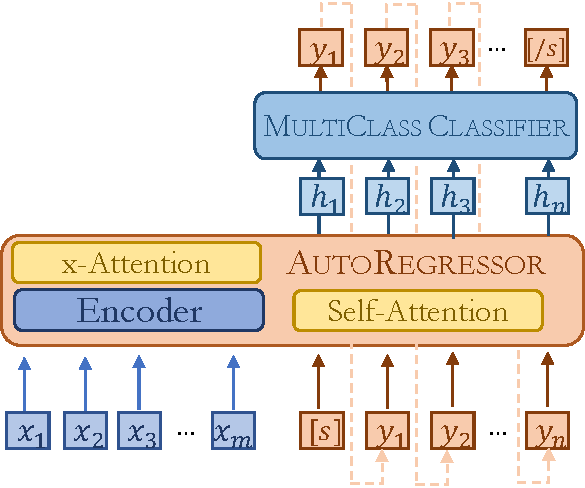
\includegraphics[width=0.65\linewidth]{img/optimvocab/nmt-arch-classifier-new}
    \caption{The NMT model re-envisioned as a token classifier with an autoregressive feature extractor.}
    \label{fig:nmt-architecture}
%% to edit this, go to https://docs.google.com/drawings/d/1Ei9m3WanLJRvoegurFZpiSRQTz7p1Mmde25G0ZwnmAU/edit 
\end{figure}

Autoregressor $R$, \cite{box2015time} being the most complex component of the NMT model, has many implementations based on various neural network architectures: recurrent neural networks (RNN) such as long short-term memory (LSTM) and gated recurrent unit (GRU), convolutional neural networks (CNN), and Transformer. 
At time step $t$, $R$ transforms the input context $y_{<t}, x_{1:m}$ into hidden state vector $h_t = R(y_{<t}, x_{1:m})$.

Classifier $C$ is the same across all architectures.
It maps $h_t$ to a distribution $P(y_j | h_t) \forall y_j \in V_Y$, where $V_Y$ is the vocabulary of $Y$. 
Input to classifiers such as $C$ is generally described as features that are either hand-engineered or automatically extracted.
In our high-level view of NMT architectures, $R$ is a neural network that serves as an automatic feature extractor for $C$.

\subsection{Balanced Classes for Token Classifier}
\label{sec:classifier-balance}

Untreated, class imbalance leads to bias based on class frequencies.
Specifically, classification learning algorithms focus on frequent classes while paying relatively less importance to infrequent classes.
Frequency-based bias leads to poor recall of infrequent classes \cite{Johnson2019SurveyImbalance}. 

When a model is used in a \textit{domain mismatch} scenario, i.e., where test and training set distributions do not match, model performance generally degrades.
It is not surprising that frequency-biased classifiers show particular degradation in domain mismatch scenarios, as  types that were infrequent in the training distribution and were ignored by the learning algorithm may appear with high frequency in the new domain.
\citet{koehn2017sixchallenges} showed empirical evidence of poor generalization of NMT to out-of-domain datasets.

In other classification tasks, where each instance is classified independently, methods such as up-sampling infrequent classes and down-sampling frequent classes are used.
In NMT, since classification is done within the context of sequences, it is possible to accomplish the objective of balancing by altering sequence lengths.
This can be done by choosing the level of subword segmentation \cite{sennrich-etal-2016-bpe}.

\textbf{Quantification of Zipfian Imbalance:}
We use two statistics to quantify the imbalance of a training distribution:

The first statistic relies on a measure of \textbf{Divergence} ($D$) from a balanced (uniform) distribution. 
We use a simplified version of Earth Mover Distance, in which the total cost for moving a probability mass between any two classes  is the sum of the total mass moved.
Since any mass moved \textit{out of} one class is moved \textit{into} another, we divide the total per-class mass moves in half to avoid double counting.  
Therefore, the imbalance measure $D$ on $K$ class distributions where $p_i$ is the observed probability of class $i$ in the training data is computed as:
$$D = \frac{1}{2} \sum_{i=1}^{K}| p_i - \frac{1}{K}|; \quad 0 \le D \le 1 $$

A lower value of $D$ is the desired setting for $C$, since the lower value results from a balanced class distribution. 
When classes are balanced, they have approximately equal frequencies; $C$ is thus less likely to make errors due to class bias.

The second statistic is \textbf{Frequency at 95th\% Class Rank (\textbf{$F_{95\%}$})}, defined as the least frequency in the $95^{th}$ percentile of most frequent classes.
More generally, $F_{\large{P\%}}$ is a simple way of quantifying the minimum number of training examples for at least the $P$th percentile of classes.
The bottom $(1-P)$ percentile of classes are ignored to avoid the noise that is inherent in the real-world natural-language datasets.

A higher value for $F_{95\%}$ is the desired setting for $C$, as a higher value indicates the presence of many training examples per class, and ML methods are known to perform better when there are many examples for each class.  


\subsection{Shorter Sequences for Autoregressor}
\label{sec:ar-short-seq}

Every autoregressive model is an approximation; some may be better than others, but no model is perfect. 
The total error accumulated grows in proportion to the length of the sequence.
These accumulated errors alter the prediction of subsequent tokens in the sequence.
Even though beam search attempts to mitigate this, it does not completely resolve it.  
These challenges with respect to long sentences and beam size are examined by \citet{koehn2017sixchallenges}.


We summarize sequence lengths using \textbf{Mean Sequence Length}, $\mu$, 
computed trivially as the arithmetic mean of the lengths of \textit{target} language sequences after encoding them:
$\mu = \frac{1}{N} \sum_{i=1}^N |y^{(i)}|$
where $y^{(i)}$ is the $i$th sequence in the training corpus of $N$ sequences.
Since shorter sequences have relatively fewer places where an imperfectly approximated autoregressor model can make errors, a smaller $\mu$ is a desired setting for $R$.

%%%%%%%%%%%%%%%%%%%%%%%%%%%%%%%%%%%%%%%%%%%%%%%%%
\subsection{Choosing the Vocabulary Size Systematically}
\label{sec:bpe}

BPE~\cite{sennrich-etal-2016-bpe} is a greedy iterative algorithm often used to segment a vocabulary into useful \textit{subwords}. 
The algorithm starts with characters as its initial vocabulary.
In each iteration, it greedily selects the most frequent type bigram in the training corpus, and replaces the sequence with a newly created compound type.
Once the subword vocabulary is learned, it can be applied to a corpus by greedily segmenting words with the longest available subword type. These operations have an effect on $D$, $F_{95\%}$, and $\mu$.

\textbf{Effect of BPE on $\mu$}:
BPE expands rare words into two or more subwords, lengthening a sequence (and raising $\mu$) relative to simple white-space segmentation.
BPE merges frequent-character sequences into one subword piece, shortening a sequence (and lowering $\mu$) relative to character segmentation.
Hence, the sequence length of BPE segmentation lies in between the sequence lengths obtained by white-space and character-only segmentation methods \cite{morishita-etal-2018-improving}. 

\textbf{Effect of BPE on $F_{95\%}$ and $D$}:
Whether BPE is viewed as a merging of frequent subwords into a relatively less frequent compound, or a splitting of rare words into relatively frequent subwords, BPE alters the class distribution by moving the probability mass of classes.
Hence, by altering the class distribution, BPE also alters both $F_{95\%}$ and $D$. The BPE hyperparameter controls the amount of probability mass moved between subwords and compounds.

Figure~\ref{fig:BPE-imbalance} shows the relation between number of BPE merges (i.e. the BPE hyperparameter), and both $D$ and $\mu$.
When few BPE merge operations are performed, we observe the lowest value of $D$, which is a desired setting for $C$, but at the same point $\mu$ is large and undesired for $R$ (Section~\ref{sec:classifier-nlg}).
When a large number of BPE merges are performed, the effect is reversed, i.e. we observe that $D$ is large and unfavorable to $C$ while $\mu$ is small and favorable to $R$. 
In the following sections we describe our experiments and analysis to locate the optimal number of BPE merges that achieves the right trade-off for both $C$ and $R$. 

 \begin{figure}[ht]
  \centering
    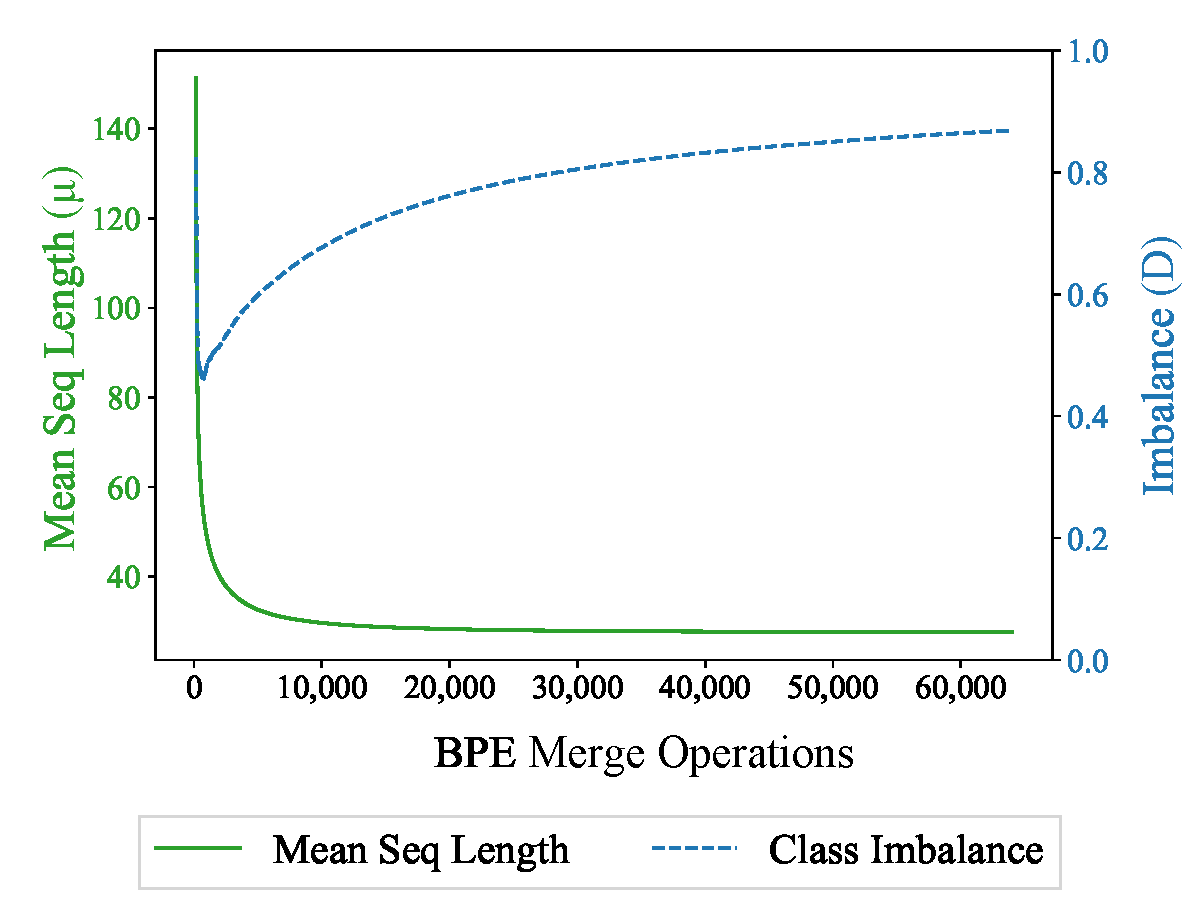
\includegraphics[width=0.7\linewidth]{bpe64k-deen-en.pdf}
    \caption{Effect of BPE merge operations on mean sequence length ($\mu$) and class imbalance ($D$).
    } 
    \label{fig:BPE-imbalance}
\end{figure}


\section{Experimental Setup}
\label{sec:exp-setup}

Our NMT experiments use the base Transformer model \cite{vaswani-2017-attention} on four different target languages at various training data sizes, described in the following subsections. 

\subsection{Datasets}
We use the following four language pairs for our analysis: English$\rightarrow$German, German$\rightarrow$English, English$\rightarrow$Hindi, and English$\rightarrow$Lithuanian. 
To analyze the impact of different training data sizes, we randomly sub-select smaller training corpora for English$\leftrightarrow$German and English$\rightarrow$Hindi language pairs. 
Statistics regarding the corpora used for validation, testing, and training are in Table~\ref{tab:datasets}.
The datasets for English$\leftrightarrow$German, and English$\rightarrow$Lithuanian are retrieved from the News Translation task of WMT2019~\cite{wmt19proceedings}.\footnote{\href{http://www.statmt.org/wmt19/translation-task.html}{http://www.statmt.org/wmt19/translation-task.html}}
For English$\rightarrow$Hindi, we use the IIT Bombay Hindi-English parallel corpus v1.5~\cite{kunchukuttan-etal-2018-iit}.
English, German, and Lithuanian sentences are tokenized using \textsc{SacreMoses}.\footnote{\href{https://github.com/alvations/sacremoses}{https://github.com/alvations/sacremoses}} 
Hindi sentences are tokenized using \textsc{IndicNlpLibrary}.\footnote{\href{https://github.com/anoopkunchukuttan/indic_nlp_library}{https://github.com/anoopkunchukuttan/indic\_nlp\_library}}

The training datasets are trivially cleaned: we exclude sentences with length in excess of five times the length of their parallel counterparts. 
Since the vocabulary is a crucial part of this analysis, we exclude all sentence pairs containing URLs. 

\begin{table*}[ht]
    \centering
    \setlength{\tabcolsep}{3pt}
\begin{tabular}{ l  : l  : r  r  r  : l : l }
  Languages & Training & Sentences & EN Toks & XX Toks & Validation & Test \\ \hline
\multirow{4}{1.5cm}{DE$\rightarrow$EN\\EN$\rightarrow$DE} 
    & \multirow{4}{4cm}{Europarl v10 \\ WMT13CommonCrawl \\ NewsCommentary v14}
         & 30K  &  0.8M & 0.8M & \multirow{4}{*}{ {\small NewsTest18} }
            & \multirow{4}{*}{ \small{NewsTest19}} \\ \cdashline{3-5}
    &    & 0.5M  & 12.9M & 12.2M &  &  \\ \cdashline{3-5}
    &    & 1M    & 25.7M & 24.3M &  &  \\ \cdashline{3-5} 
    &    & 4.5M  & 116M & 109.8M &  &  \\ \hdashline

\multirow{2}{*}{EN$\rightarrow$HI } 
     & \multirow{2}{*}{ IITB Training } 
         & 0.5M & 8M & 8.6M  & \multirow{2}{*}{ \small{IITB Dev} } 
     & \multirow{2}{*}{ \small{IITB Test} }  \\\cdashline{3-5} 
     &   & 1.3M & 21M & 22.5M   &   &  \\ \hdashline 
EN$\rightarrow$LT & Europarl v10 & 0.6M & 17M & 13.4M  & \small{NewsDev19} & \small{NewsTest19} \\
\end{tabular} 
    \caption{Training, validation, and testing datsets, along with sentence and token counts in training sets. We generally refer to dataset's sentences as size in this chapter.}
    \label{tab:datasets}
\end{table*}

\subsection{Hyperparameters}
Our model is a 6 layer Transformer encoder-decoder that has 8 attention heads, 512 hidden vector units, and a feed forward intermediate size of 2048, with GELU activation. 
We use label smoothing at 0.1, and a dropout rate of 0.1.
We use the Adam optimizer \cite{kingma2015adam} with a controlled learning rate that warms up for 16K steps followed by the decay rate recommended for training Transformer models~\cite{popel2018tfm-train-tips}. 
To improve performance at different data sizes, we set the mini-batch size to 6K tokens for the 30K-sentence datasets, 12K tokens for 0.5M-sentence datasets, and 24K for the remaining larger datasets~\cite{popel2018tfm-train-tips}. 
All models are trained until no improvement in validation loss is observed, with patience of 10 validations, each done at 1,000 update steps apart. 
Our model is implemented using PyTorch and run on NVIDIA P100 and V100 GPUs.
To reduce padding tokens per batch, mini-batches are made of sentences having similar lengths \cite{vaswani-2017-attention}.
We trim longer sequences to a maximum of 512 tokens after BPE.
To decode, we average the last 10 checkpoints, and use a beam size of 4 with length penalty of 0.6, similar to \citet{vaswani-2017-attention}.

Since the vocabulary size hyperparameter is the focus of this analysis, we use a range of vocabulary sizes that include character vocabulary and BPE operations that yield vocabulary sizes between 500 and 64K types.
A common practice, as seen in \citet{vaswani-2017-attention}'s setup, is to jointly learn BPE for both source and target languages, which facilitates three-way weight sharing between the encoder's input, the decoder's input, and the output (i.e., classifier's class) embeddings \cite{press-wolf-2017-embeddings}.
However, to facilitate fine-grained analysis of vocabulary sizes and their effect on class imbalance, our models separately learn source and target vocabularies; weight sharing between the encoder's and decoder's embeddings is thus not possible.
For the target language, however, we share weights between the decoder's input and the classifier's class embeddings.

\section{Results and Analysis}
\label{sec:nmt_analysis}

\begin{figure}[h!t]
\centering
\begin{subfigure}{\linewidth}
    \centering
    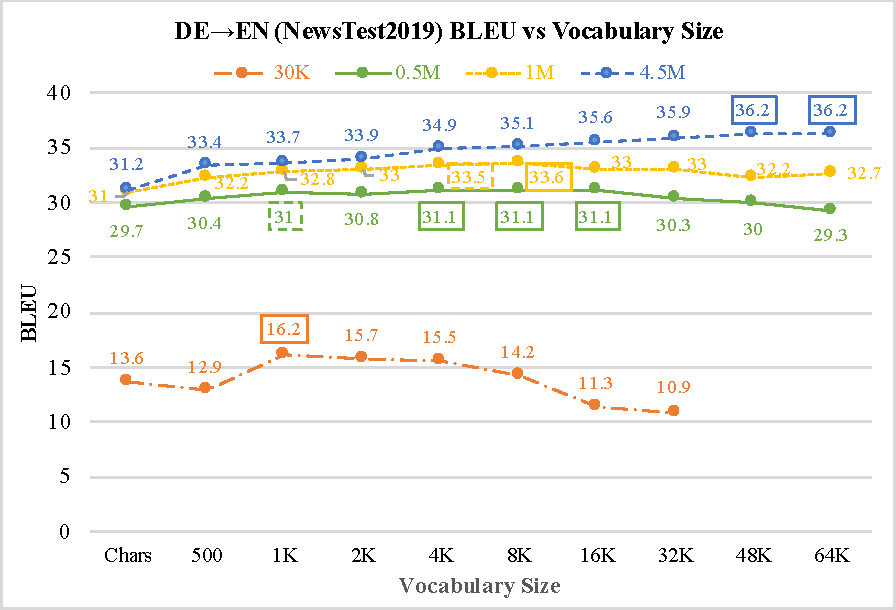
\includegraphics[width=0.7\linewidth]{bleu-deen.pdf}
    \caption{DE$\rightarrow$EN BLEU on NewsTest2019}
    \label{fig:bleu-deen}
\end{subfigure}

\vspace{5mm}

\begin{subfigure}{\linewidth}
    \centering
    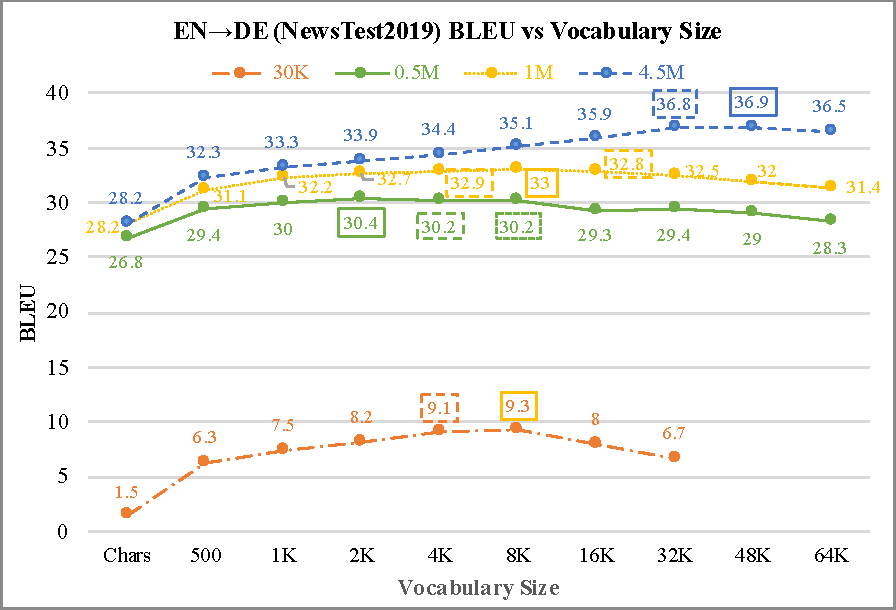
\includegraphics[width=0.7\linewidth]{bleu-ende.pdf}
    \caption{EN$\rightarrow$DE BLEU on NewsTest2019}
    \label{fig:bleu-ende}
\end{subfigure}
\caption{EN$\leftrightarrow$DE NewsTest2019 BLEU as a function of vocabulary size at various training set sizes. 
Only the large dataset with 4.5M sentences has its best performance at a large vocabulary; all others peak at an 8K or smaller vocabulary size.}
\label{fig:bleu-ende-deen}
\end{figure}

\begin{figure}[ht]
    \centering    
    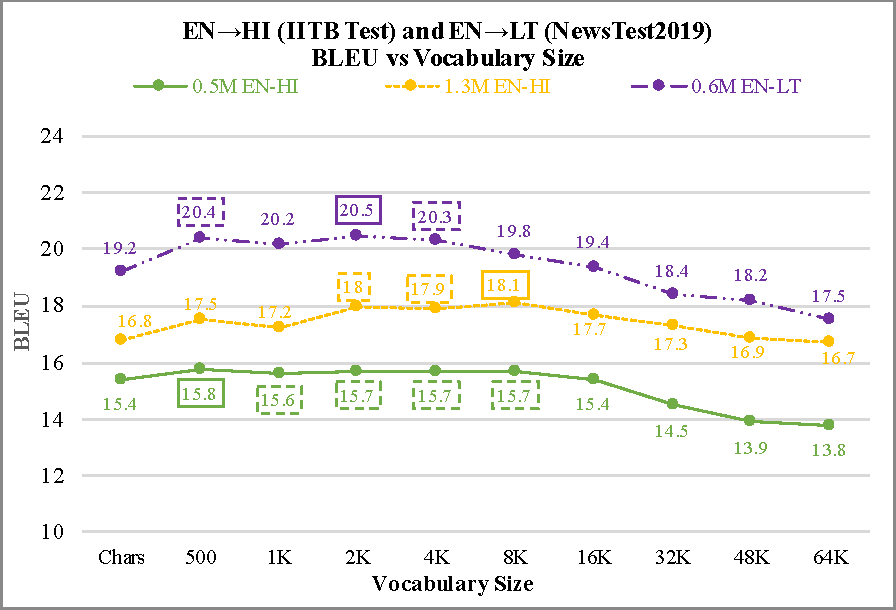
\includegraphics[width=0.7\linewidth]{bleu-enhi-enlt.pdf}
    \caption{BLEU on EN$\rightarrow$HI IITB Test and EN$\rightarrow$LT NewsTest2019 as a function of vocabulary size.
    These language pairs observed the best BLEU scores in the range of 500 to 8K vocabulary size.}
    \label{fig:bleu-enhilt}
\end{figure}

BLEU scores for DE$\rightarrow$EN and EN$\rightarrow$DE experiments are reported in Figures~\ref{fig:bleu-deen} and \ref{fig:bleu-ende} respectively.
Results from EN$\rightarrow$HI, and EN$\rightarrow$LT are combined in Figure~\ref{fig:bleu-enhilt}.
All the reported BLEU scores are obtained using \textsc{SacreBleu} \cite{post-2018-sacrebleu}.\footnote{\texttt{BLEU+case.mixed+numrefs.1+smooth.exp+tok.13a+version.1.4.6}}

We make the following observations: smaller vocabulary such as characters have not produced the best BLEU for any of our language pairs or dataset sizes. 
A vocabulary of 32K or larger is unlikely to produce optimal results unless the data set is large e.g. the 4.5M DE$\leftrightarrow$EN sets.
The BLEU curves as a function of vocabulary sizes have a shape resembling a hill. 
The position of the peak of the hill seems to shift towards a larger vocabulary when the datasets are large. 
However, there is a lot of variance in the position of the peak: one extreme is at 500 types on 0.5M EN$\rightarrow$HI, and the other extreme is at 64K types in 4.5M DE$\rightarrow$EN. 
    
Although Figures~\ref{fig:bleu-ende-deen} and \ref{fig:bleu-enhilt} indicate \textit{where} the optimal vocabulary size is for these chosen language pairs and datasets, the question of \textit{why} the peak is where it is remains unanswered.
We visualize $\mu$, $D$, and $F_{95\%}$ in Figures \ref{fig:mu-d-freq-bleu} and \ref{fig:mu-d-freq-bleu-continued} to answer that question, and report these observations:
\begin{enumerate}
    \itemsep0em 
    \item Small vocabularies have a relatively larger $F_{95\%}$ (favorable to classifier), yet they are suboptimal. We reason that this is due to the presence of a larger $\mu$, which is unfavorable to the autoregressor.
    \item Larger vocabularies such as 32K and beyond have a smaller $\mu$, which favors the autoregressor, yet rarely achieves the best BLEU.
    We reason this is due to the presence of a lower $F_{95\%}$ and a higher $D$ being unfavorable to the classifier.
    Since the larger datasets have many training examples for each class, as indicated by a generally larger $F_{95\%}$, we conclude that bigger vocabularies tend to yield optimal results compared to smaller datasets in the same language.
    
    \item On small (30K) to medium (1.3M) data sizes, the vocabulary size of 8K seems to find a good trade-off between $\mu$ and $D$, as well as between $\mu$ and $F_{95\%}$.
\end{enumerate}

 There is a \textit{simple heuristic} to locate the peak: the near-optimal vocabulary size is where sentence length $\mu$ is small, while $F_{95\%}$ is approximately $100$ or higher.
 
 
 \begin{figure}[h!t]
    \centering
    \begin{subfigure}{0.8\textwidth}
    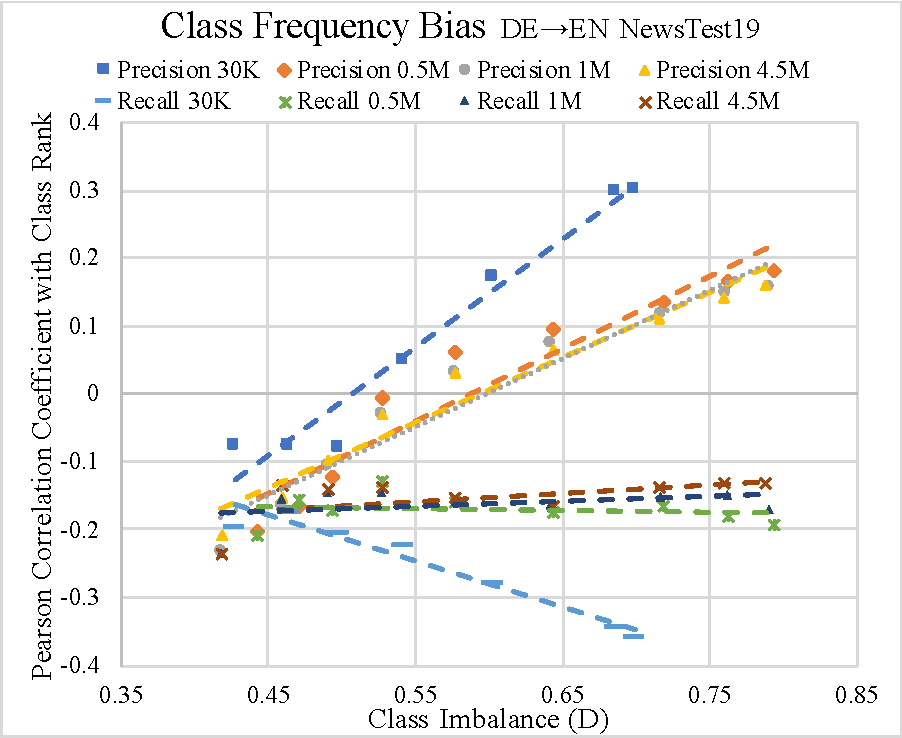
\includegraphics[width=\linewidth]{corr-deen-test.pdf}
    \end{subfigure}
    
    \vspace{5mm}

    \begin{subfigure}{0.8\textwidth}
    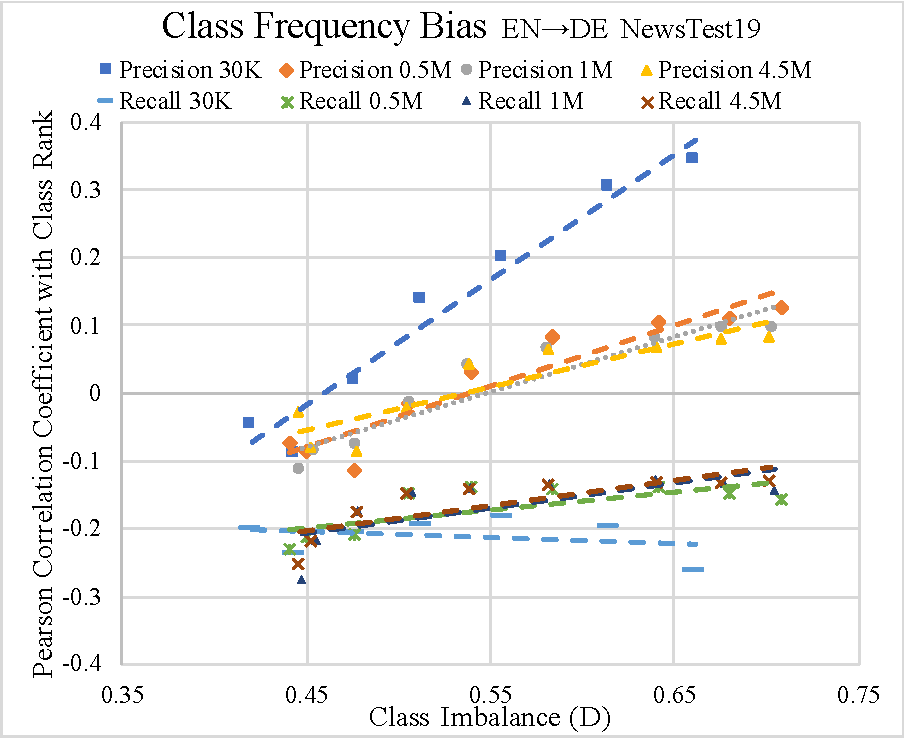
\includegraphics[width=\linewidth]{corr-ende-test.pdf}
    \end{subfigure}
    
    \caption{Correlation analysis on DE$\rightarrow$EN and EN$\rightarrow$DE shows that NMT models suffer from frequency based class bias, indicated by non-zero correlation of both precision and recall with class rank. Reduction in class imbalance (D), as shown by the horizontal axis, generally reduces the bias as indicated by the reduction in magnitude of correlation.}
         \label{fig:corr-deen-test}
\end{figure}
 
 

\begin{figure}[h!t]
\centering
\begin{subfigure}{\textwidth}
  \centering
  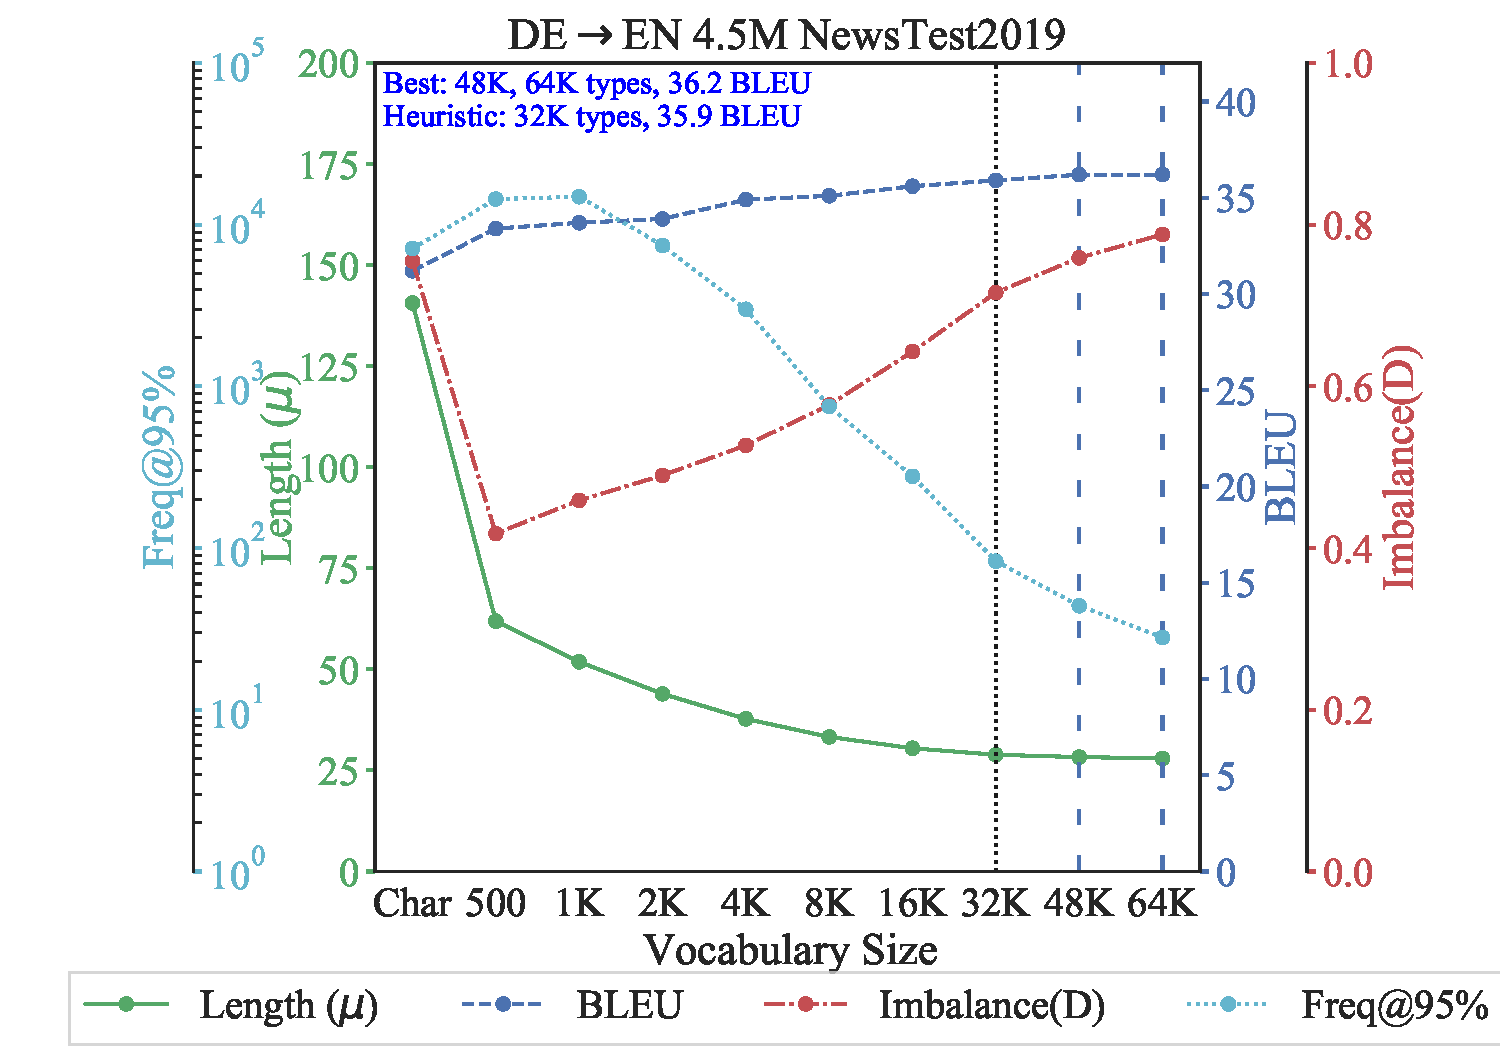
\includegraphics[width=0.7\linewidth,trim={1.4cm 0 0.2cm 16.45cm},clip]{4axv-test-deen-4.5m.pdf}
\end{subfigure}

\vspace{1mm}

\begin{subfigure}{.44\textwidth}
  \centering
  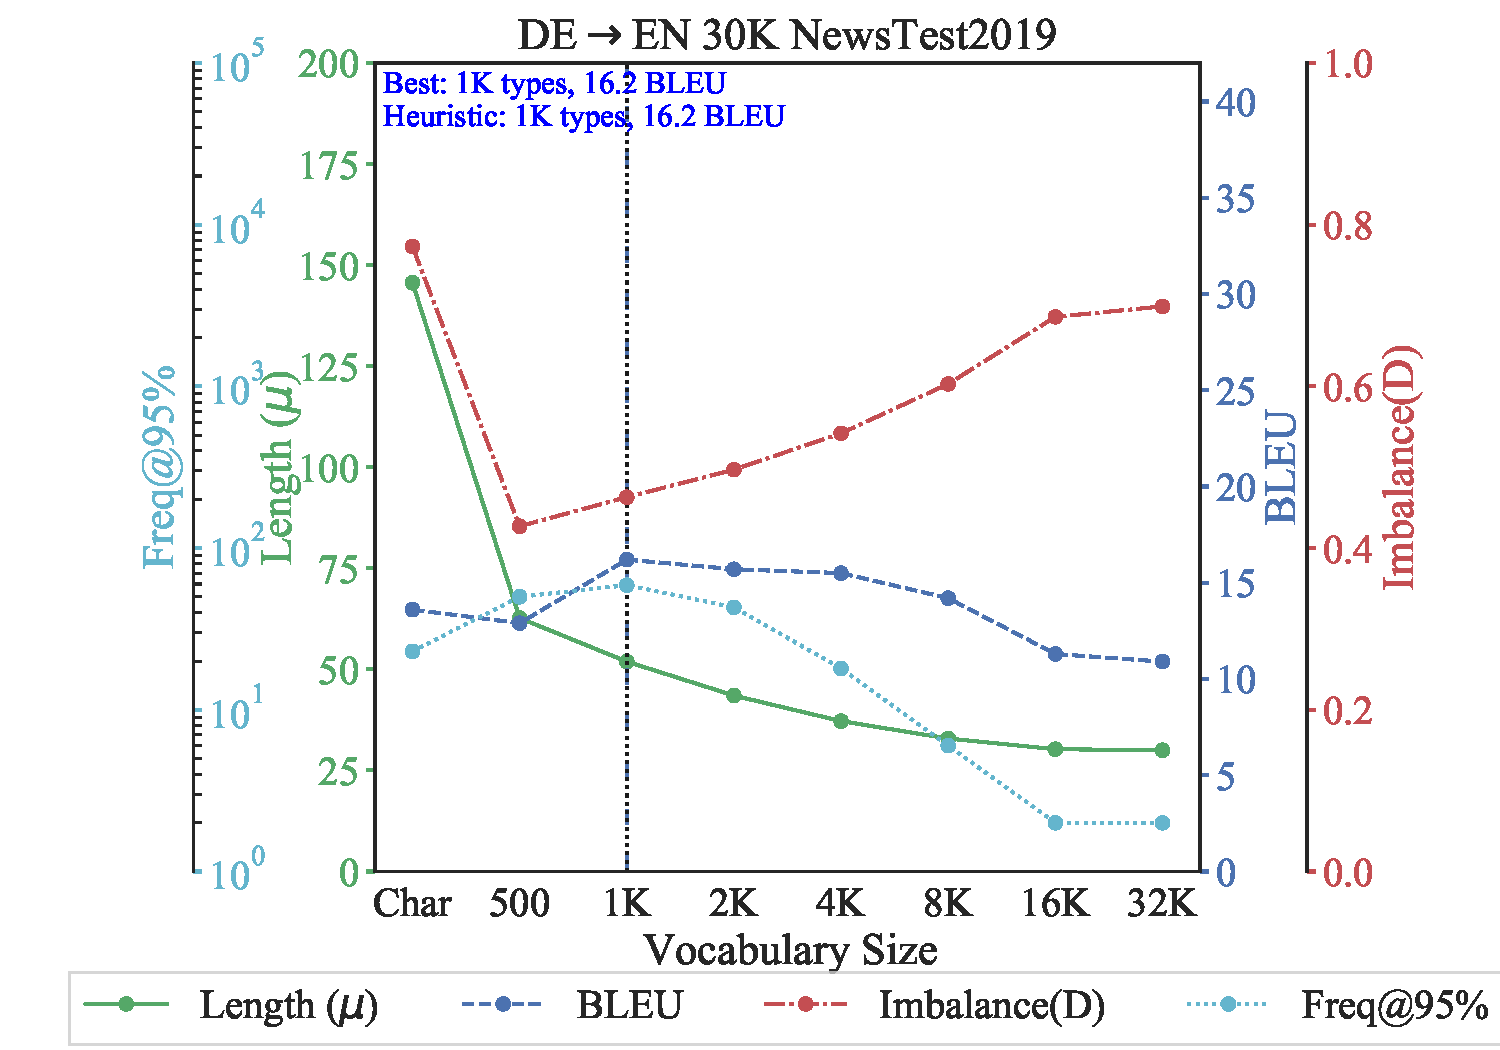
\includegraphics[width=0.99\linewidth,trim={2.4cm 1.32cm 4.1cm 0},clip]{4axv-test-deen-30k.pdf}
  %\caption{1a}
  %\label{fig:sfig1}
\end{subfigure}
\begin{subfigure}{.44\textwidth}
  \centering
  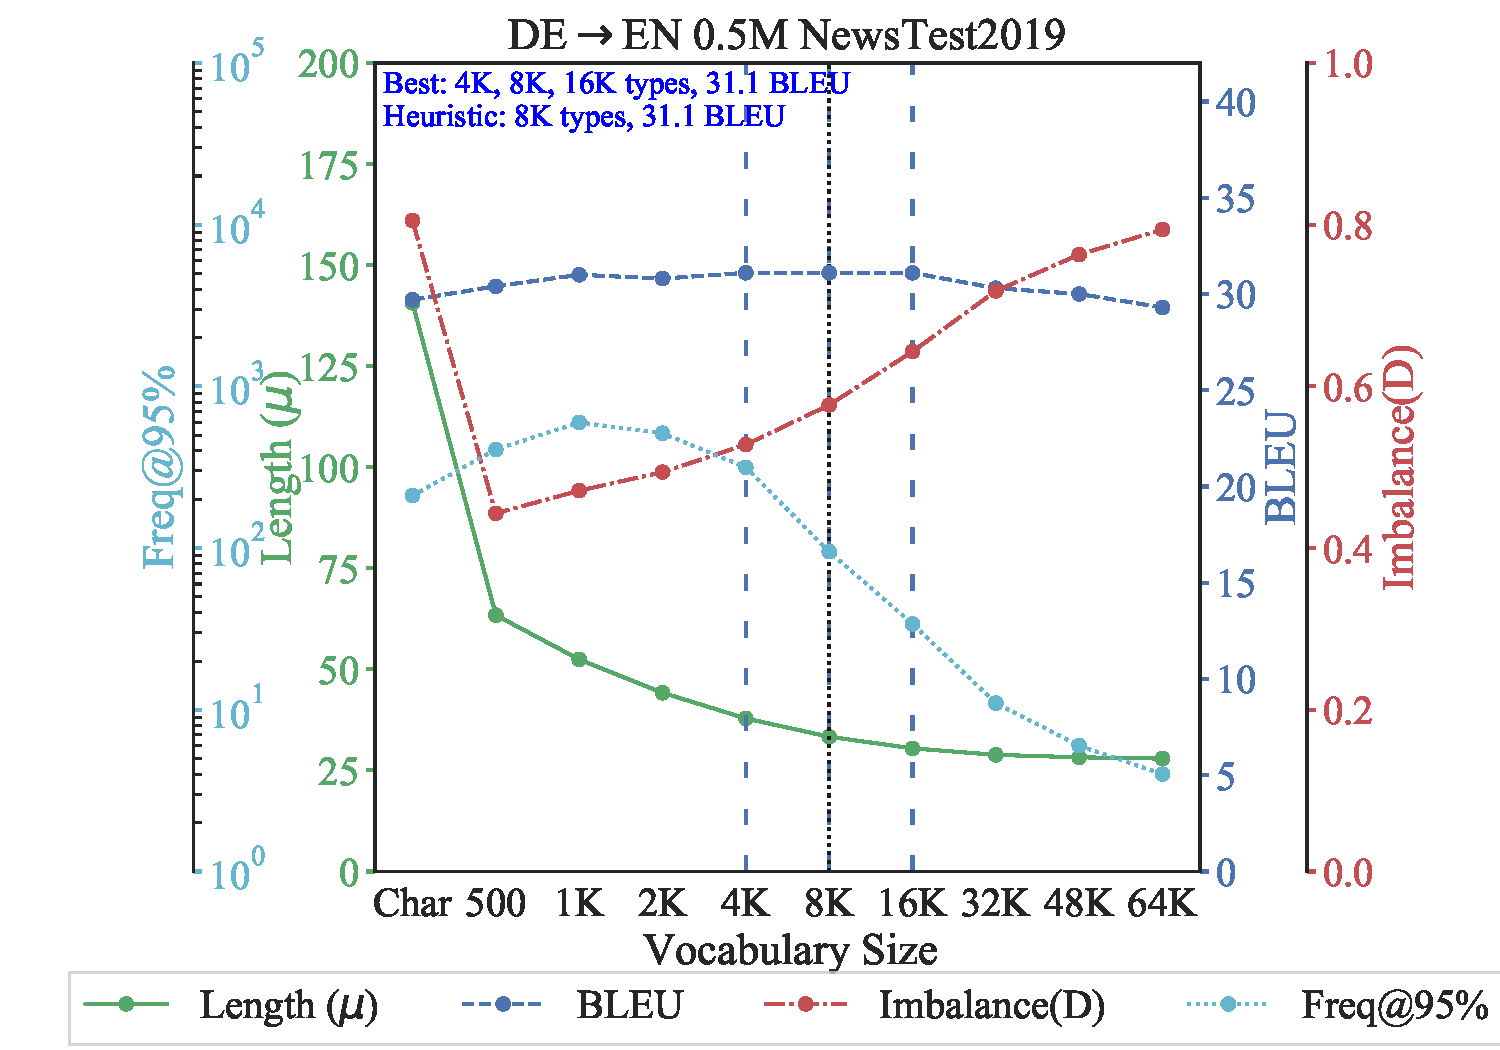
\includegraphics[width=0.99\linewidth,trim={5.1cm 1.32cm 1.4cm 0},clip]{4axv-test-deen-0.5m.pdf}
  %\caption{1c}
  %\label{fig:sfig2}
\end{subfigure}


\begin{subfigure}{.44\textwidth}
  \centering
  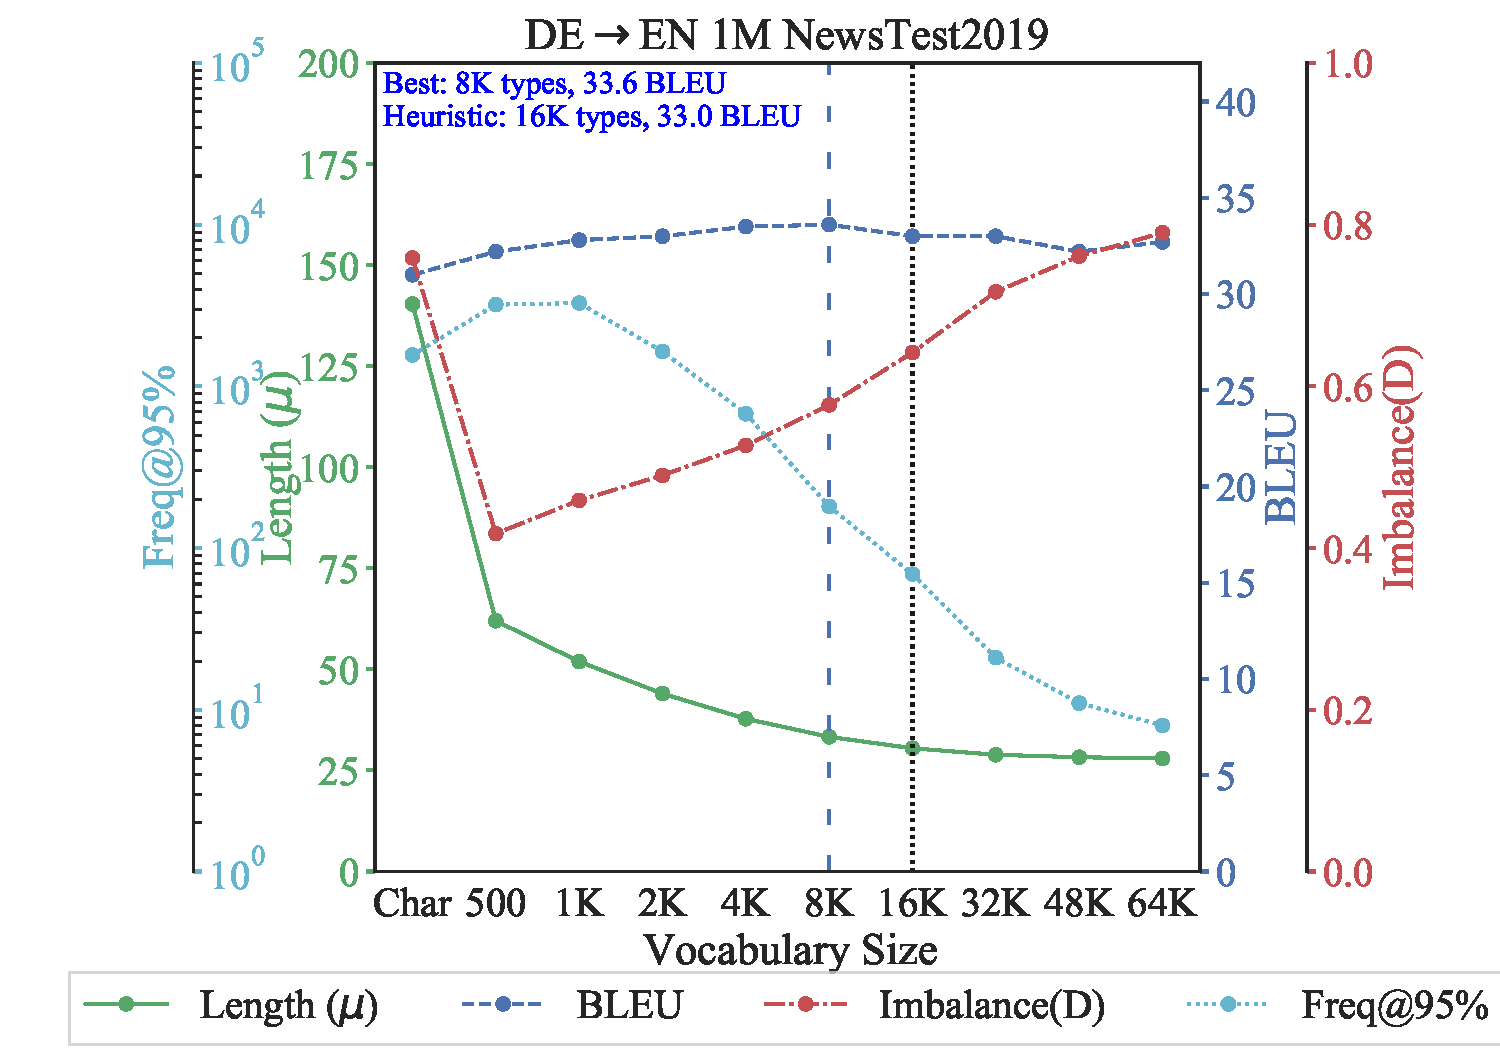
\includegraphics[width=0.99\linewidth,trim={2.4cm 1.32cm 4.1cm 0},clip]{4axv-test-deen-1m.pdf}
  %\caption{1c}
  %\label{fig:sfig2}
\end{subfigure}
\begin{subfigure}{.44\textwidth}
  \centering
  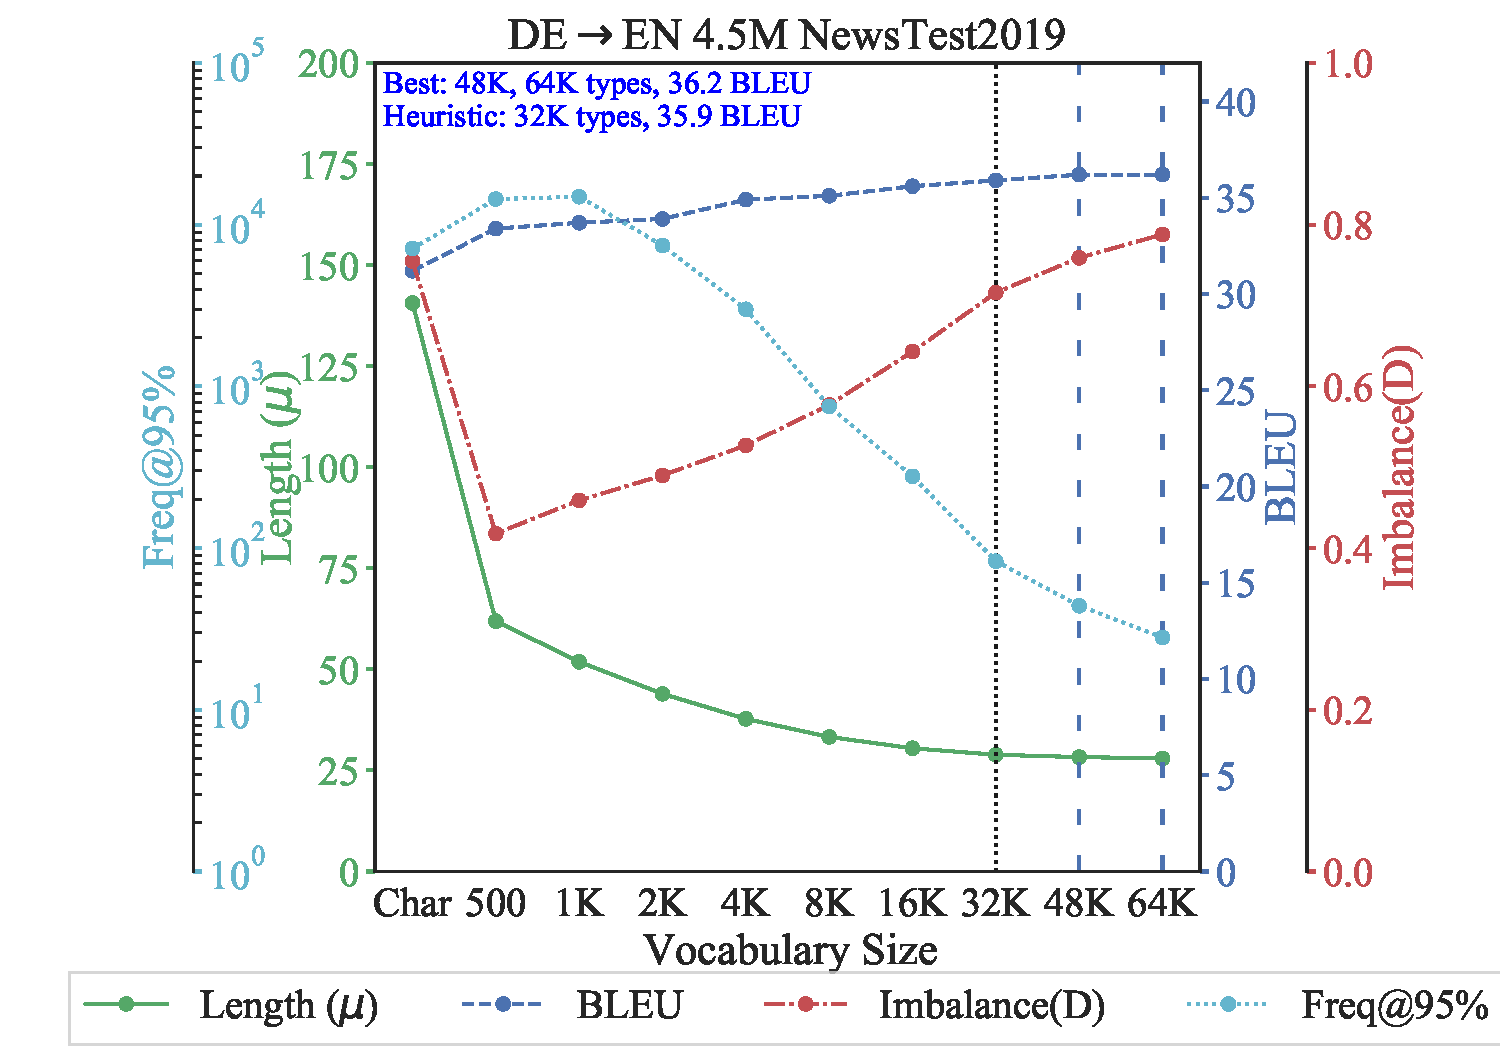
\includegraphics[width=0.99\linewidth,trim={5.1cm 1.32cm 1.4cm 0},clip]{4axv-test-deen-4.5m.pdf}
  %\caption{1c}
  %\label{fig:sfig2}
\end{subfigure}

\begin{subfigure}{.44\textwidth}
  \centering
  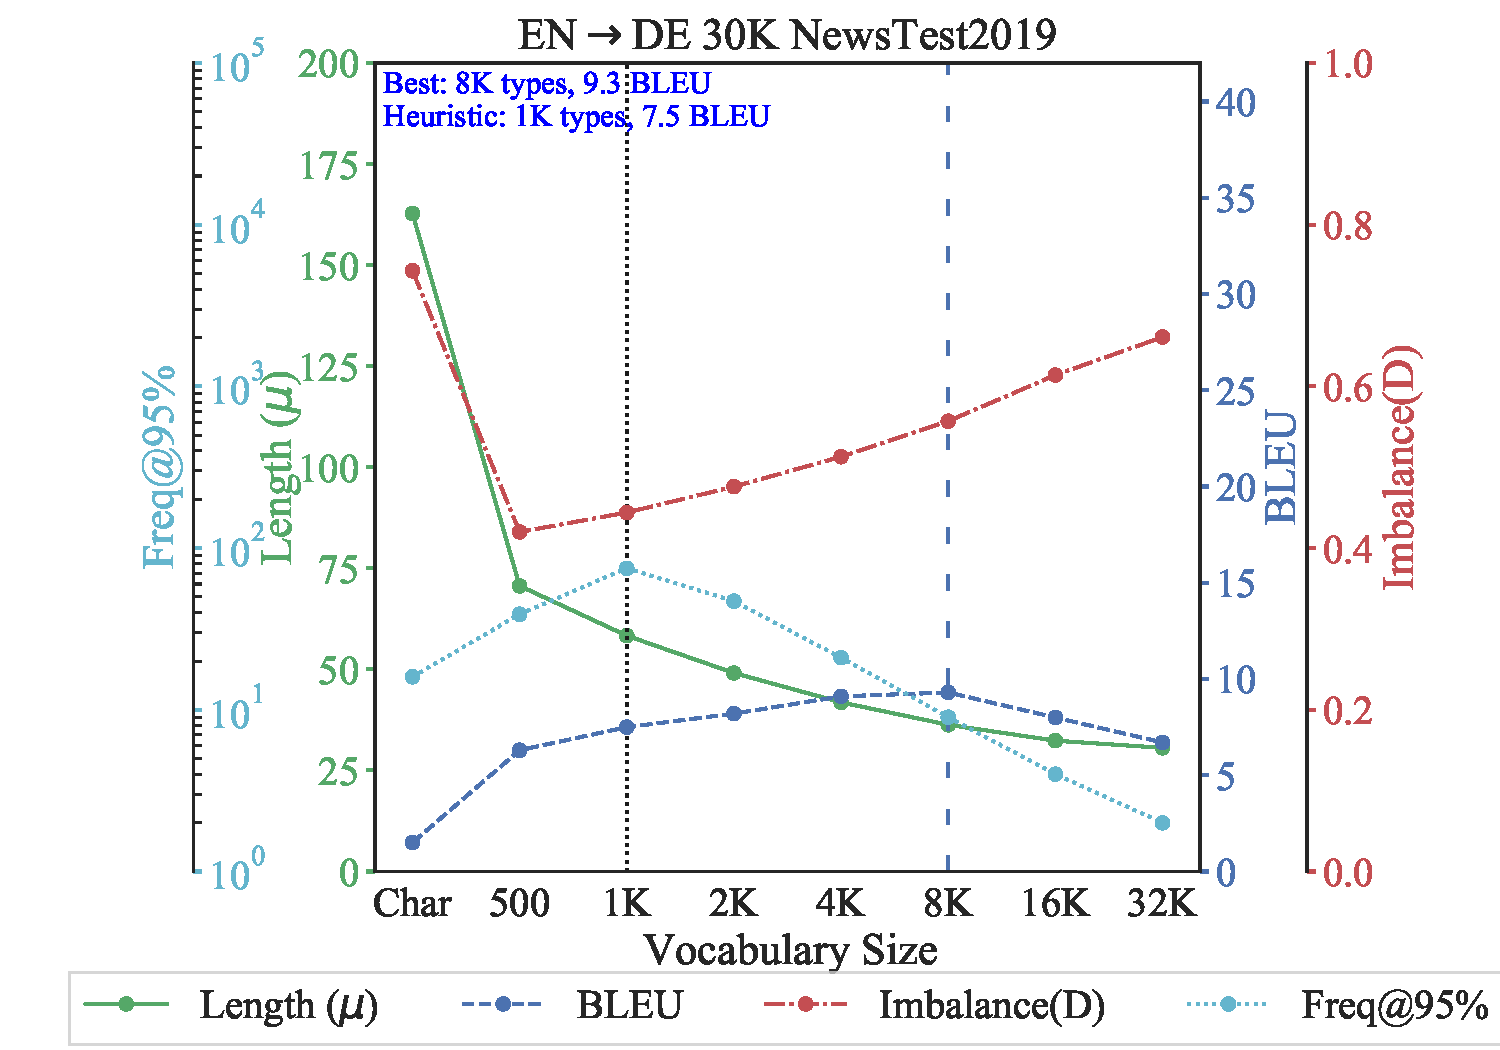
\includegraphics[width=0.99\linewidth,trim={2.4cm 1.32cm 4.1cm 0},clip]{4axv-test-ende-30k.pdf}
 % \caption{1a}
  %\label{fig:sfig1}
\end{subfigure}
\begin{subfigure}{.44\textwidth}
  \centering
  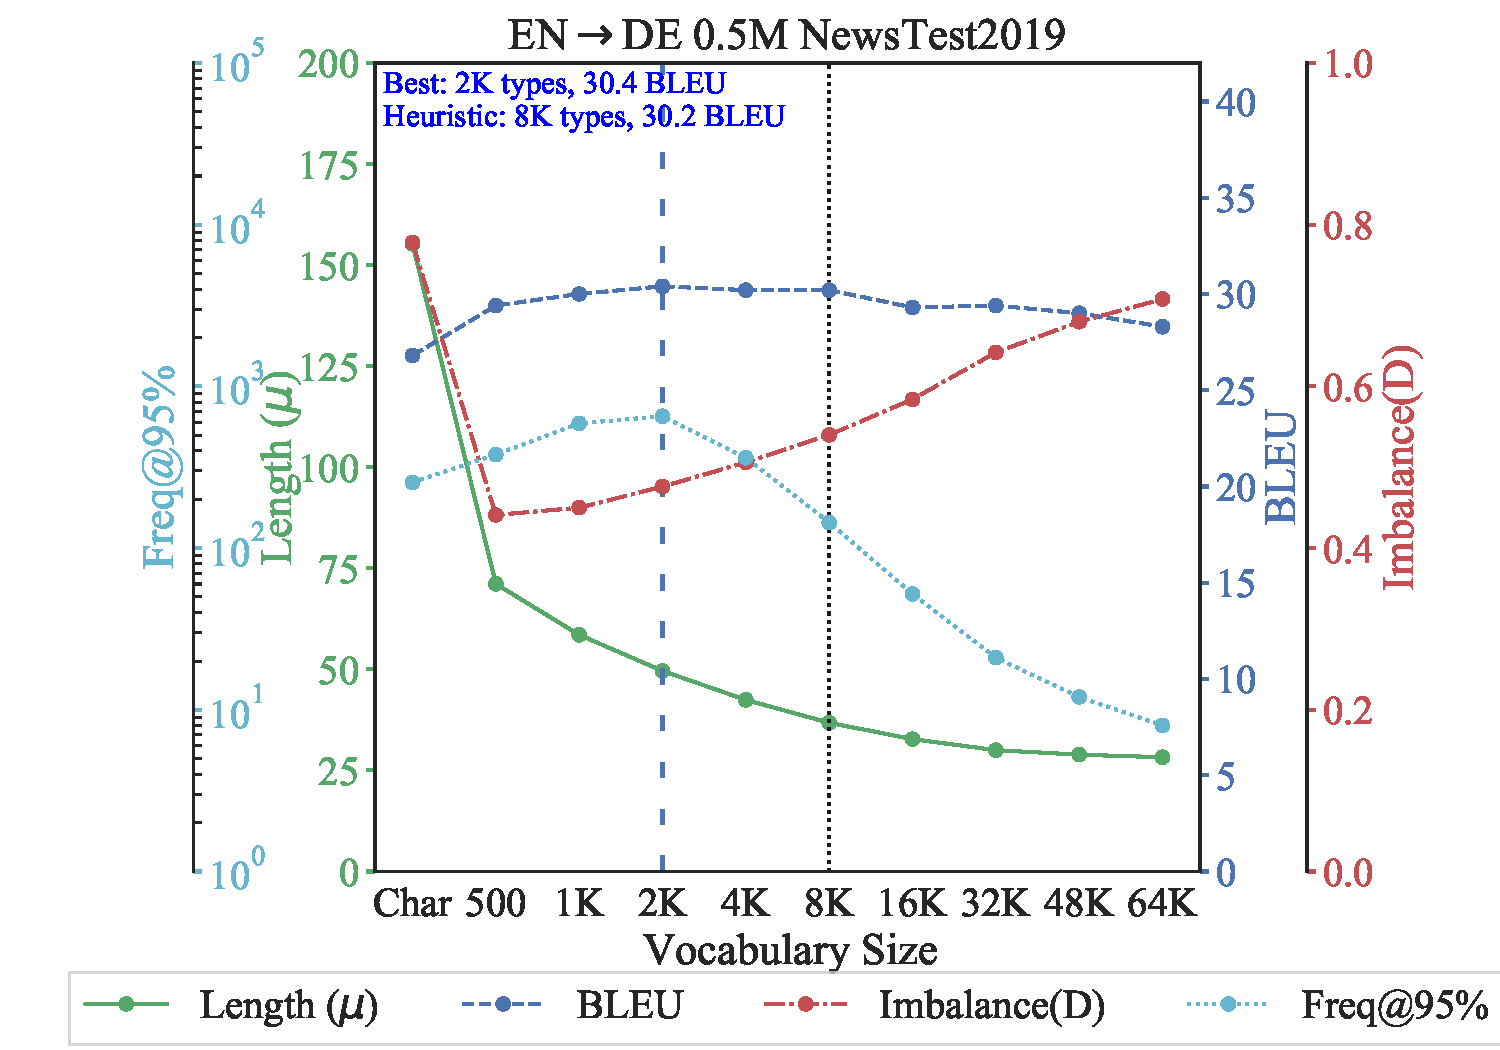
\includegraphics[width=0.99\linewidth,trim={5.1cm 1.32cm 1.4cm 0},clip]{4axv-test-ende-0.5m.pdf}
  %\caption{1c}
  %\label{fig:sfig2}
\end{subfigure}

\caption[Visualization of sequence length, class imbalance, frequency of $95^{th}$ percentile class, and test set BLEU.]{Visualization of sequence length ($\mu$) (lower is better), class imbalance (D) (lower is better), frequency of $95^{th}$ percentile class ($F_{95\%}$) (higher is better; plotted in logarithmic scale), and test set BLEU (higher is better) on all language pairs and training data sizes.
%DE$\leftrightarrow$EN of 1M resembles resembles DE$\leftrightarrow$EN of 0.5M and is provided in Appendix~\ref{sec:appendix} along with visualizations on validation sets.
The vocabulary sizes that achieved highest BLEU are indicated with dashed vertical lines, and the vocabulary our heuristic selects is indicated by dotted vertical lines.}
\label{fig:mu-d-freq-bleu}
\end{figure}

\begin{figure}[h!t]
\ContinuedFloat
\centering

\begin{subfigure}{\textwidth}
  \centering
  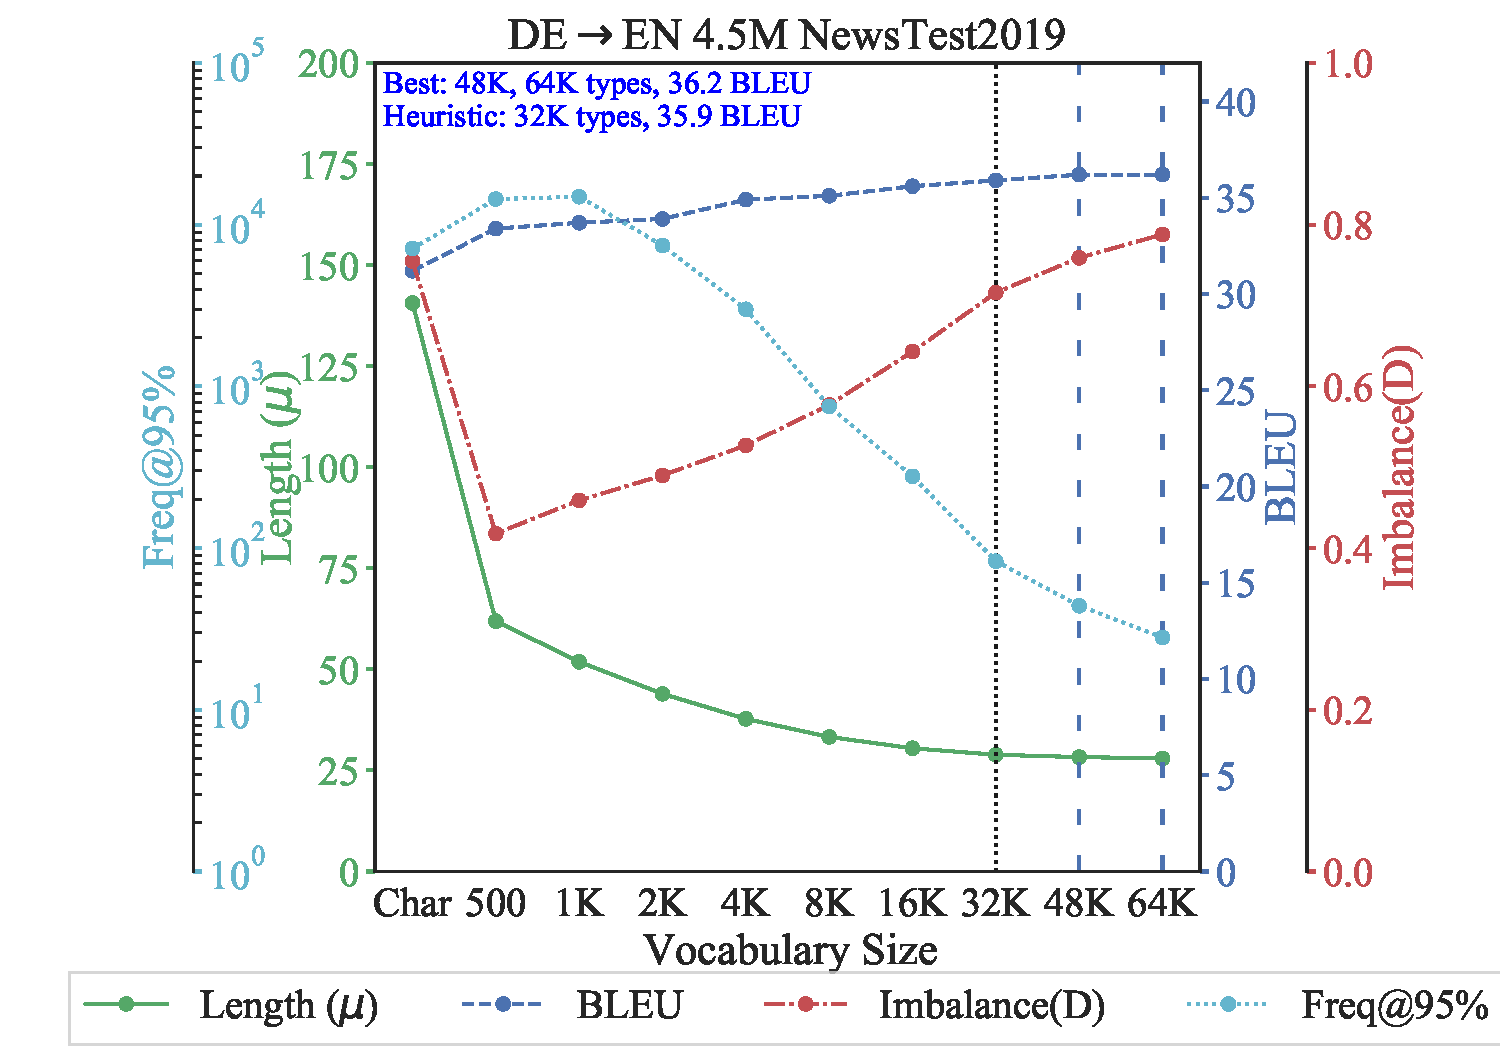
\includegraphics[width=0.7\linewidth,trim={1.4cm 0 0.2cm 16.45cm},clip]{4axv-test-deen-4.5m.pdf}
\end{subfigure}

\vspace{2mm}

\begin{subfigure}{.45\textwidth}
  \centering
  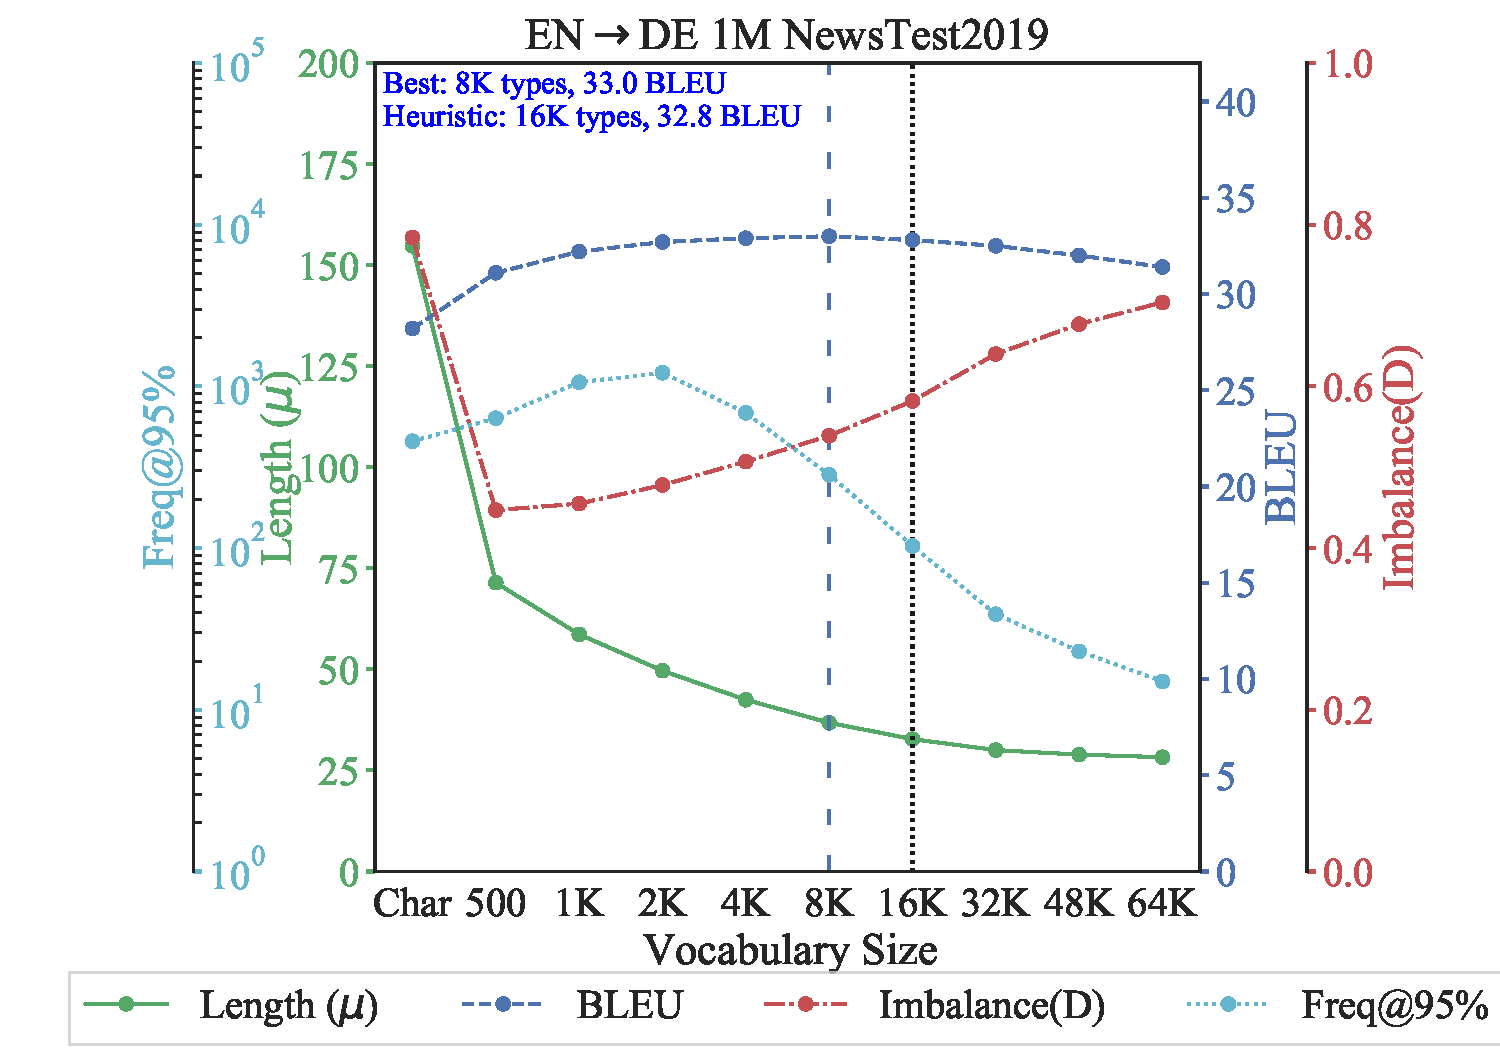
\includegraphics[width=0.99\linewidth,trim={2.4cm 1.32cm 4.1cm 0},clip]{4axv-test-ende-1m.pdf}
 % \caption{1c}
  %\label{fig:sfig2}
\end{subfigure}
\begin{subfigure}{.45\textwidth}
  \centering
  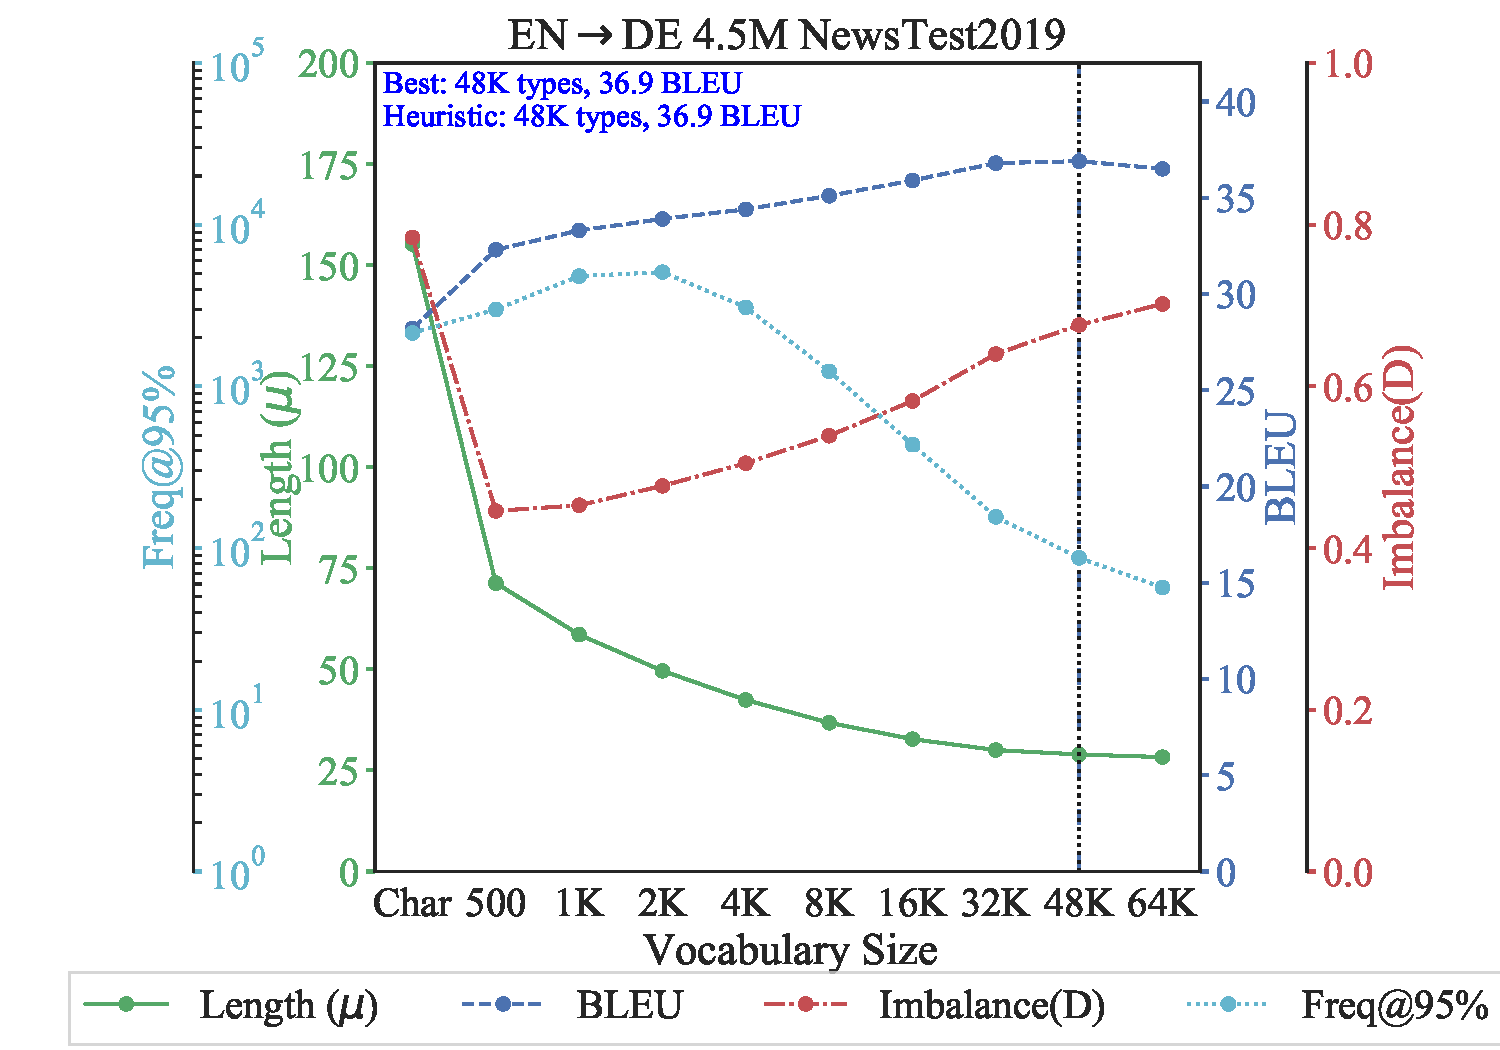
\includegraphics[width=0.99\linewidth,trim={5.1cm 1.32cm 1.4cm 0},clip]{4axv-test-ende-4.5m.pdf}
 % \caption{1c}
  %\label{fig:sfig2}
\end{subfigure}


\begin{subfigure}{.45\textwidth}
  \centering
  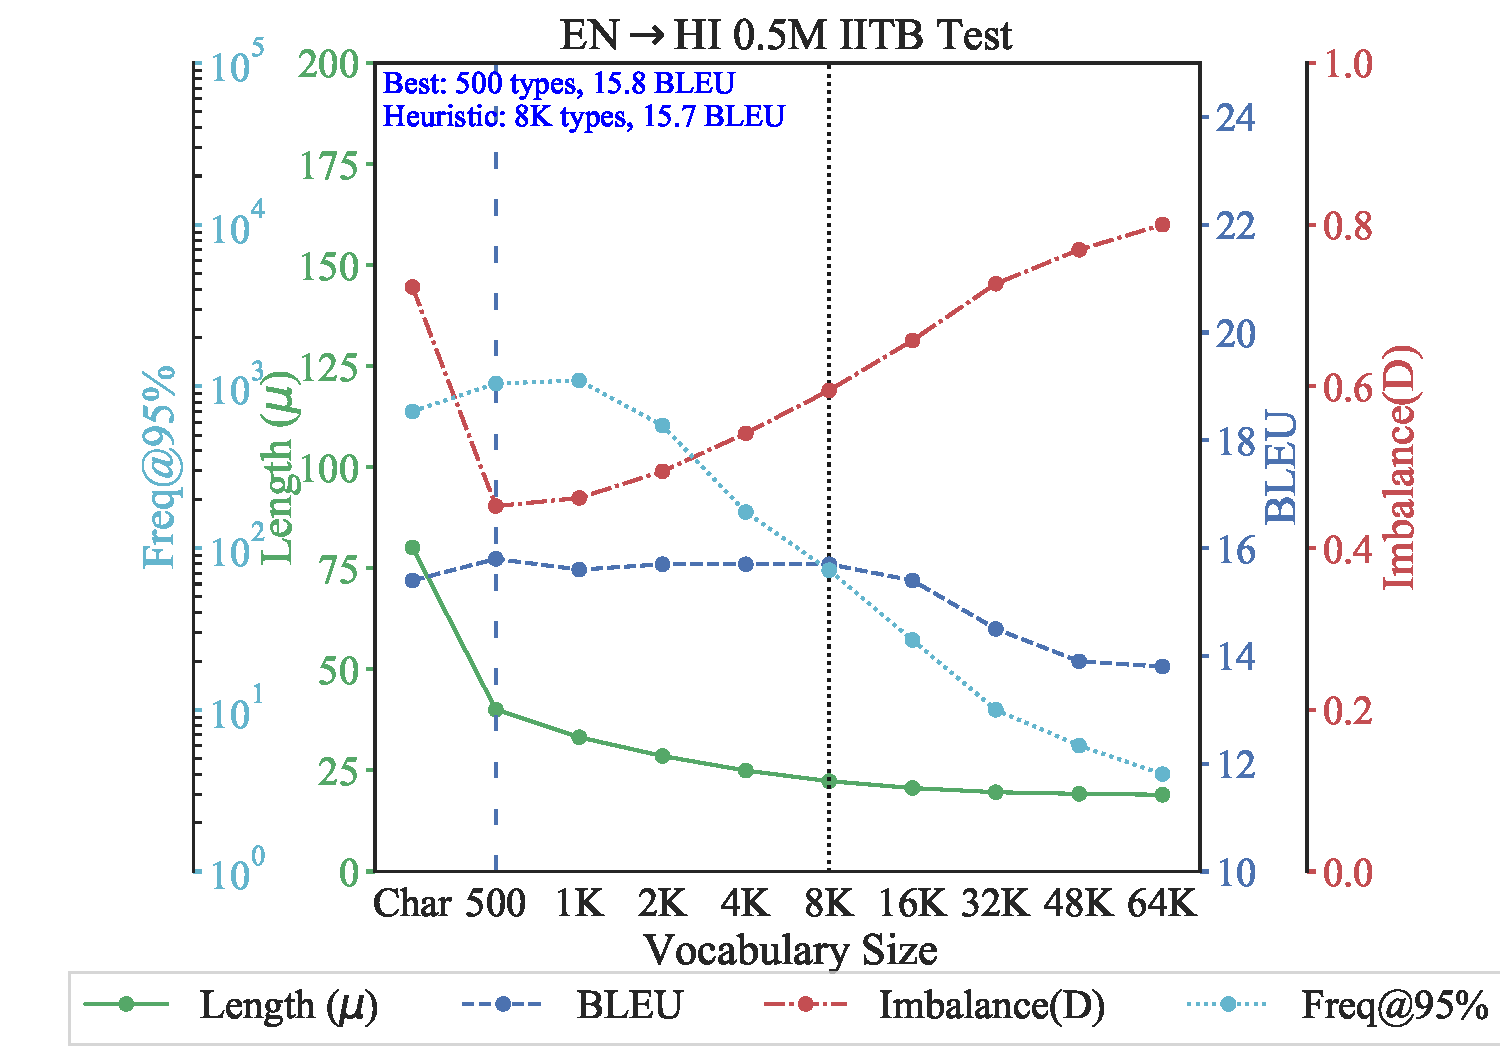
\includegraphics[width=0.99\linewidth,trim={2.4cm 1.32cm 4.1cm 0},clip]{4axv-test-enhi-0.5m.pdf}
 % \caption{1a}
  %\label{fig:sfig1}
\end{subfigure}
\begin{subfigure}{.45\textwidth}
  \centering
  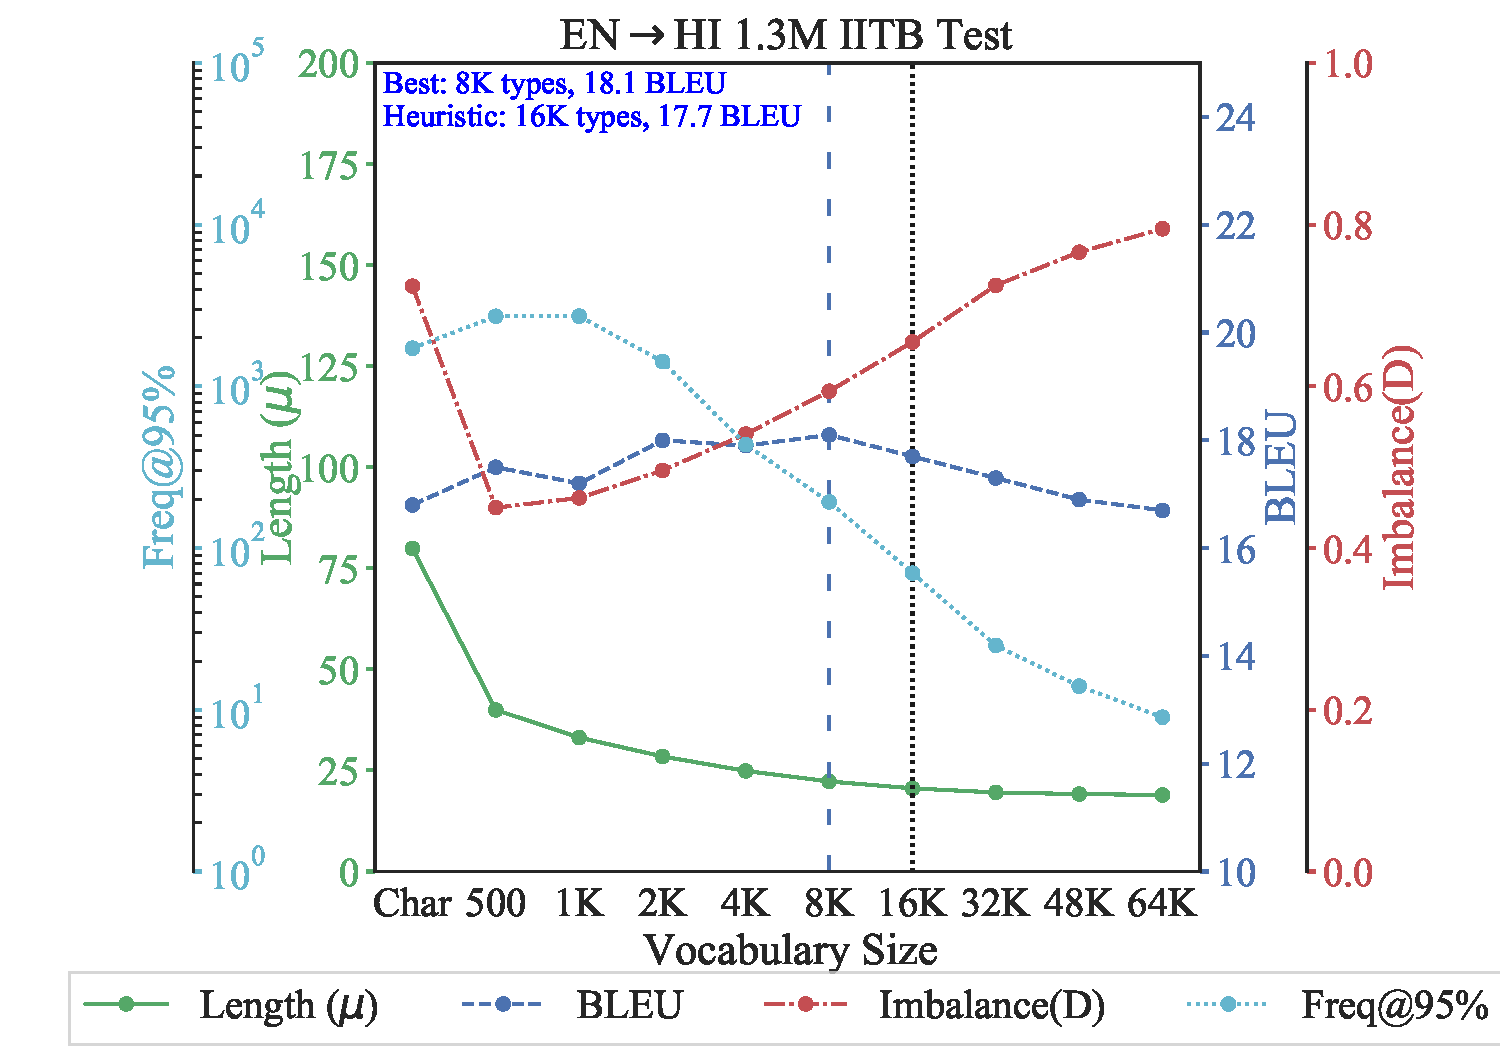
\includegraphics[width=0.99\linewidth,trim={5.1cm 1.32cm 1.4cm 0},clip]{4axv-test-enhi-1.3m.pdf}
  %\caption{1c}
  %\label{fig:sfig2}
\end{subfigure}

\begin{subfigure}{.54\textwidth}
  \centering
  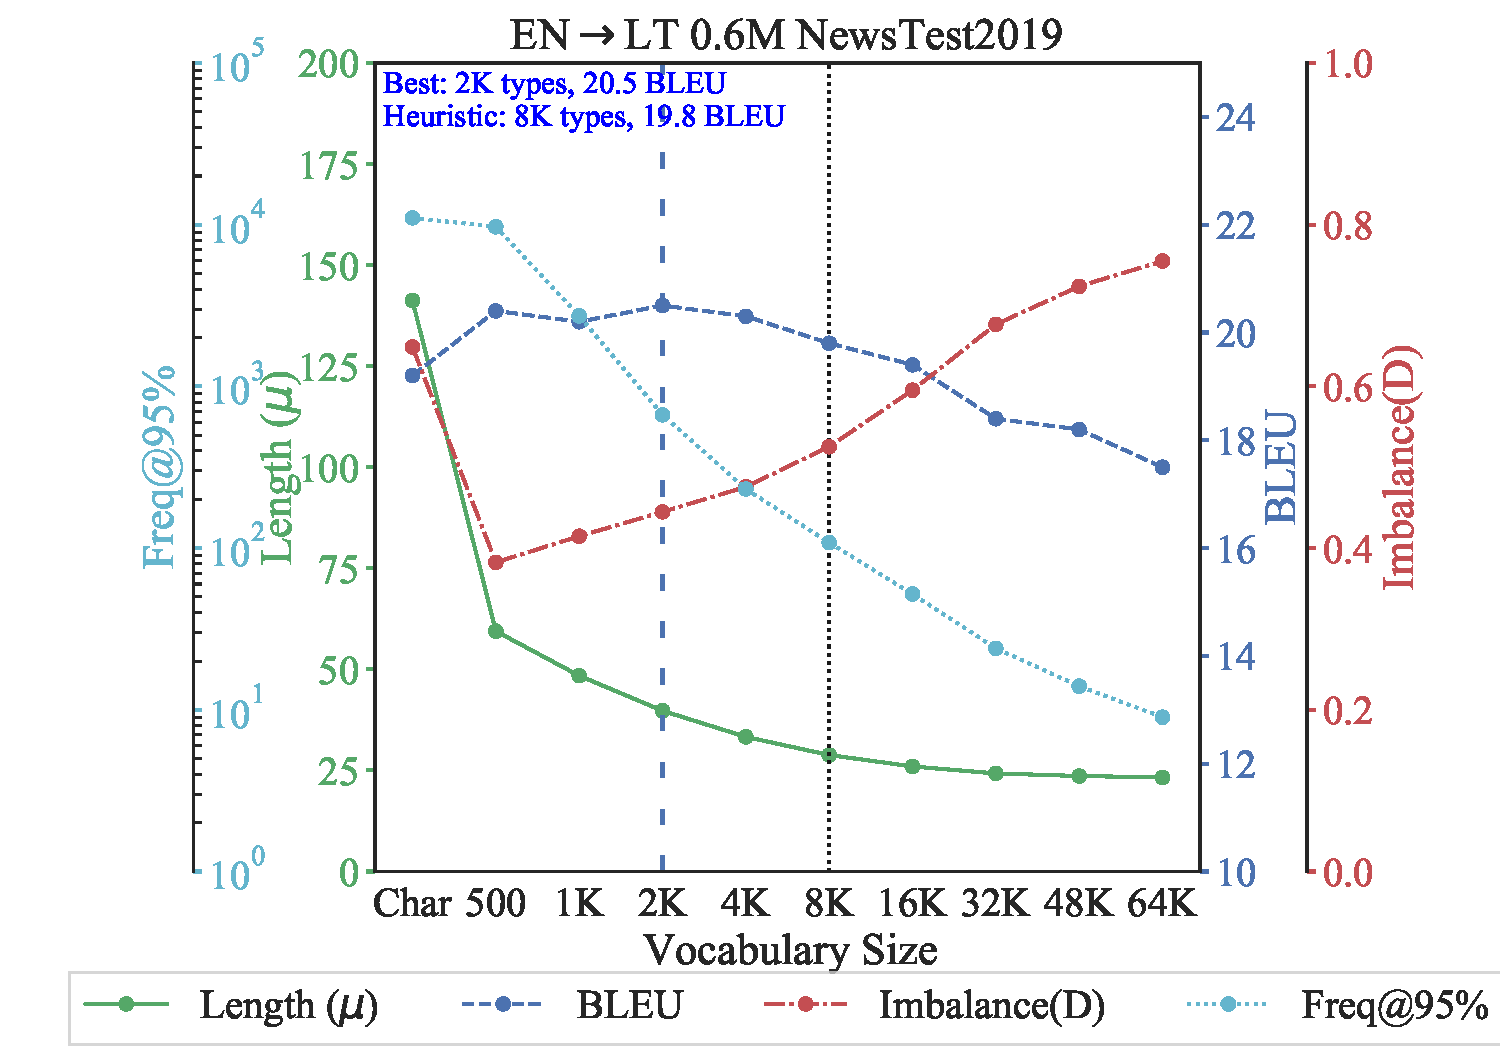
\includegraphics[width=0.99\linewidth,trim={2.4cm 1.32cm 1.4cm 0},clip]{4axv-test-enlt-0.6m.pdf}
  %\caption{1c}
  %\label{fig:sfig2}
\end{subfigure}

\caption{Continuation of Figure~\ref{fig:mu-d-freq-bleu} (see previous page for caption)}
\label{fig:mu-d-freq-bleu-continued}
\end{figure}

BLEU scores are often lower at larger vocabulary sizes---where $\mu$ is (favorably) low but $D$ is (unfavorably) high (Figure~\ref{fig:mu-d-freq-bleu}). This calls for a further investigation that is discussed in the following section.

\section{Measuring Classifier Bias Due to Imbalance}
\label{sec:class-bias}

In a typical classification setting with imbalanced classes, the classifier learns an undesired bias based on frequencies. 

A balanced class distribution debiases in this regard, leading to improvement in the precision of frequent classes as well as recall of infrequent classes.
However, BLEU focuses only on the \textit{precision} of classes; except for adding a global brevity penalty, it is ignorant of the poor recall of infrequent classes. 

Therefore, the BLEU scores shown in Figures~\ref{fig:bleu-deen}, \ref{fig:bleu-ende} and \ref{fig:bleu-enhilt} capture only a part of the improvements and biases. 
In this section, we perform a detailed analysis of the impact of class balancing by considering both precision \textit{and} recall of classes. 

We accomplish this in two stages:
First, we define a method to measure the bias of the model for classes based on their frequencies.
Second, we track the bias in relation to vocabulary size and class imbalance, and report DE$\rightarrow$EN, as it has many data points.

\subsection{Frequency Based Bias}
We measure frequency bias using the Pearson correlation coefficient, $\rho$, between class rank and class performance, while for performance measures we use precision and recall.
Classes are ranked based on descending order of frequencies in the training data, encoded with the same encoding schemes used for reported NMT experiments.
With this setup, the class with rank 1, say $F_1$, is the one with the highest frequency, rank 2 is the next highest, and so on.
More generally, $F_c$ is an index in the class rank list which has an inverse relation to class frequencies.

Following our definitions in Section~\ref{ch:background-sec:eval}, we compute precision ($P_c$) and recall ($R_c$) for each class $c$.
The Pearson correlation coefficients between class rank and precision ($\rho_{F, P}$), and class rank and recall ($\rho_{F, R})$ are reported in Figure \ref{fig:corr-deen-test}.
In datasets where $D$ is high, the performance of classifier correlates with class rank. Such correlations are undesired for a classifier.


\subsection{Analysis of Class Frequency Bias}
An ideal classifier is one that does not discriminate classes based on their frequencies, i.e., one that exhibits no correlation between $\rho_{F, P}$, and$\rho_{F, R}$.  
However, we see in Figure~\ref{fig:corr-deen-test} that:
\begin{enumerate}
    \itemsep0em
    \item $\rho_{F, P}$ is positive when the dataset has high $D$; i.e. if the class rank increases (frequency decreases), precision increases in relation to it.
    This indicates that frequent classes have relatively less precision than infrequent classes.
    The bias is strongly positive on smaller datasets such as 30K DE$\rightarrow$EN, which gradually diminishes if the training data size is increased or a vocabulary setting is chosen to reduce $D$.
    \item $\rho_{F, R}$ is negative, i.e., if the class rank increases, recall decreases in relation to it. 
    This is an indication that infrequent classes have relatively lower recall than frequent classes.
\end{enumerate}
Figure~\ref{fig:corr-deen-test} shows a trend that frequency based bias measured by correlation coefficient is lower in settings that have lower $D$.
However, since $D$ is non-zero, there still exists non-zero correlation between recall and class rank ($\rho_{F, R}$), indicating the poorer recall of low-frequency classes.

%%%%%%%%%%%%%%%%%%%%%%%%%%%%%%%%%%%%%%%%%%%%%%%%%%%%%%%%%%%%%%%%%%%%%%%%%%%%
\section{Conclusion}
\label{sec:conclusion}
Envisioning NMT as a multi-class classifier with an autoregressor helps in analyzing its weaknesses.
Our analysis provides an explanation of \textit{why} text generation using BPE vocabulary is more effective compared to word and character vocabularies, and \textit{why} certain BPE hyperparameters are better than others.
We show that the number of BPE merges is not an arbitrary hyperparameter, and that it can be tuned to address the class imbalance and sequence length problems. 
Our recommendation for Transformer NMT is to \textit{use the largest possible BPE vocabulary, such that at least 95\% of classes have 100 or more examples in training}.
Even though certain BPE vocabulary sizes indirectly reduce the class imbalance, they do not completely eliminate it.
The class distributions after applying BPE contain sufficient imbalance for inducing the frequency based bias, especially affecting the recall of rare classes. 
Hence, more effort in the future is needed to directly address the Zipfian imbalance.

%\section*{Acknowledgments}
%This research is based upon work supported in part by the Office of the Director of National Intelligence (ODNI), Intelligence Advanced Research Projects Activity (IARPA), via contract \# FA8650-17-C-9116, and by research sponsored by Air Force Research Laboratory (AFRL) under agreement number FA8750-19-1-1000. The views and conclusions contained herein are those of the authors and should not be interpreted as necessarily representing the official policies, either expressed or implied, of ODNI, IARPA, Air Force Laboratory, DARPA, or the U.S. Government. The U.S. Government is authorized to reproduce and distribute reprints for governmental purposes notwithstanding any copyright annotation therein.